% !TeX spellcheck = en_US
%Publications.tex
%\newcommand{\PublicationsPath}{PatentsAndPublications/Publications}

%IEEECOMST2021

\section[A Survey on Virtual Network Functions for Media Streaming: Solutions and Future Challenges]{A Survey on Virtual Network Functions for Media Streaming: Solutions and Future Challenges}
\label{chap:IEEECOMST2021}
\begin{itemize} \itemsep1pt\parskip0pt\parsep0pt
	\item \textbf{Title:} A Survey on Virtual Network Functions for Media Streaming: Solutions and Future Challenges
	\item \textbf{Authors:} Roberto~Viola, \'Angel~Mart\'in, Mikel~Zorrilla, Jon~Montalb\'an, Pablo~Angueira and Gabriel-Miro~Muntean
	\item \textbf{Journal:} IEEE Communications Surveys and Tutorials
	\item \textbf{Publisher:} IEEE
	\item \textbf{Year:} (Submitted May 5, 2021)
%	\item \textbf{DOI:}  \url{}
\end{itemize}	
	
\textbf{Abstract:} Media streaming services rely heavily on good and predictable network performance when delivered to large numbers of people. Media services need to ensure enhanced user perceived quality levels during content playback to attract and retain audiences, especially while the streams are distributed remotely via networks. Furthermore, as the quality of media content gets higher, the network performance demands are also increasing and it is challenging to meet them. To this end, Content Delivery Networks (CDN) employ diverse solutions to empower media streaming, including \hbox{state-of-the-art} streaming technologies, such as HTTP Adaptive Streaming (HAS). Network functions should help to further enhance media streaming services and cope with the high dynamics of network performance and user mobility. Furthermore, new networking paradigms and architectures under the 5G networks umbrella are bringing new possibilities to deploy smart network functions, which monitor the media streaming services through live and objective metrics and boost them in real time. This survey overviews the state-of-the-art technologies and solutions proposed to apply new network functions for enhancing quality of service (QoS), quality of experience (QoE) and other business and energy metrics in the context of media streaming.
	
\textbf{Keywords:} Media streaming, network functions, quality of service, network virtualization, network traffic, network forecast.
		
\subsection{Introduction}
\label{sec:IEEECOMSTintro}
	
In the recent years, media streaming traffic is constantly growing. 
Wireless and mobile devices are becoming main sources for both rich media content generation and consumption. 5G networks must cope with this new traffic demand supporting higher bandwidth and reduced latency. It is estimated that 5G connections will handle nearly three times more traffic than a current LTE connection by 2023 \cite{Cisco2020}.
New applications involving video streams are gaining relevance and are attracting an increased audience, including in areas in which there was little or no rich media presence. Examples of professional applications and application areas which can benefit from advanced media streaming include Industrial Internet of Things (IIoT), medical equipment and connected and autonomous vehicles.
Moreover, 3D video formats enable support for new services, such as eXtended Reality (XR), Virtual Reality (VR) and Augmented Reality (AR). Finally, online gaming and video conferencing are also highly popular, especially in the last period. These services have increasing demands in terms of network support. However, although the networks have growing capabilities, there is a large increase in rich media streaming traffic, mostly fueled by the global COVID-19 pandemic. This pandemic is transforming users' habits to access the Internet \cite{Lutu2020, Feldmann2020} and media content consumption \cite{Favale2020, King2020}. The Broadband Commission for Sustainable Development, a joint initiative of the International Telecommunication Union (ITU) and the United Nations Educational, Scientific and Cultural Organization (UNESCO), is also concerned about these user habit changes and it is implementing an Agenda for Action to push an emergency response to the pandemic, aiming at Internet access extension and boosting its capacity \cite{BroadbandCommission, ICTaffordability}.

All the above-mentioned factors are inevitably influencing the evolution of all services, and especially affect the rich media ones. It is therefore evident that there is a need for new network-related solutions to support high quality of service (QoS) for these applications. The current network traffic crosses networks working on a best-effort basis where no details regarding packet delivery (e.g., time) is guaranteed. Therefore, best-effort networked-transmitted media traffic may result in lower user quality of experience (QoE). A paradigmatic example of this QoE degradation are stalls or artifacts during media playback on player devices. Employing content delivery networks (CDNs) is the most common solution to prevent negative quality effects and make video delivery more efficient. CDNs are geographically distributed hierarchical systems that cache and store video streams to foster efficiency and increase the service coverage. CDN price is decreasing, but the overall cost for the content provider is increasing, as the traffic from/to CDN is increasing \cite{Rayburn2020}.

Beyond CDNs, more advanced solutions based on Network Function Virtualization (NFV) technologies \cite{Han2015} are being investigated to support media streaming services. NFV allows the deployment of Virtual Network Functions (VNF) devoted to empower network abilities when delivering media streaming traffic in an optimized and cost-effective manner \cite{Jahromi2018, Dieye2018}. VNFs enable flexible operations whose benefits are threefold. First, VNF-based networks monitor objective operational parameters, such as throughput or latency, representative for QoS of the media streaming dataflows, which have a direct influence on user satisfaction.
However, QoS metrics do not perfectly map on user experience, as user perceived quality is highly subjective. Additionally, QoE which compiles subjective evaluation elements, including rewards for playback quality and smoothness, and penalties for image freezes and unstable or low quality \cite{Kim2010, Alreshoodi2013}, needs to be considered, too.
Secondly, the Content Provider (CP) has more control to shape the network traffic and allocate resources since business rules for VNF deployment and life-cycle management could be established. These rules allow balancing network resources and business costs trade-offs \cite{Hernandez2015}, so they are highly relevant.
Last, as the volume, complexity and real-time nature of the media streaming traffic has an evident impact on energy consumption of the network and devices managing the content, an optimized streaming delivery through VNFs should also consider the energy efficiency.
	
	
In this context, the main contributions of this survey are:
\begin{itemize}
	\item The survey discusses widely employed performance assessment solutions and metrics related to media streaming. Metrics are classified into four subgroups: QoS, QoE and fairness, business metrics and energy efficiency;
	\item The survey provides an extensive overview of the literature involving media traffic monitoring and analysis, including traffic characterization and analysis to enable forecasts. Most common tools for network performance monitoring and simulation are also presented;
	\item The survey analyzes and classifies the \hbox{state-of-the-art} performance-driven network functions for media streaming;
	\item The survey presents technologies considered by the telecommunications industry as key enablers for the next generation networks, and discusses remaining challenges.
\end{itemize}

\begin{longtable}{p{0.2\textwidth}p{0.7\textwidth}}
%	\centering
	\caption{List of Acronyms used in the paper.}
		\label{tab:IEEECOMSTacronyms}\\
	\hline
	3GPP & 3rd Generation Partnership Project \\
	5G & Fifth Generation \\
	6G & Sixth Generation \\
	AES & Advanced Encryption Standard \\
	AES-CBC & AES block cipher mode \\
	AES-CTR & AES counter mode \\
	ANN & Artificial Neural Network \\
	AR & Augmented Reality \\
	% BSS & Business System Support \\
	C-RAN & Cloud-RAN \\
	CAPEX & Capital Expenditure \\
	CDN & Content Delivery Network \\
	CSI & Channel State Information \\
	CMAF & Common Media Application Format \\
	CN & Core Network \\
	COTS & Commercial off-the-shelf \\
	CP & Content Provider \\
	% CQI & Channel Quality Indicator \\
	CRM & Customer Relationship Management \\
	DASH & Dynamic Adaptive Streaming over HTTP \\
	DNS & Domain Name System \\
	% DTLS & Datagram Transport Layer Security \\
	DTN & Delay-tolerant Networking \\
	% EM & Element Management \\
	ESN & Echo State Network \\
	ETSI & European Telecommunications Standards Institute \\
	FeMBMS & Further enhanced MBMS \\
	GUI & Graphical User Interface \\
	HAS & HTTP Adaptive Streaming \\
	HLS & HTTP Live Streaming \\
	HTTP & HyperText Transfer Protocol \\
	IaaS & Infrastructure as a Service \\
	IBN & Intent-Based Network \\
	IoT & Internet of Things \\
	IIoT & Industrial Internet of Things \\
	IM & Instant Messaging \\
	IP & Internet Protocol \\
	ISP & Internet Service Provider \\
	ITU & International Telecommunication Union \\
	KPI & Key Performance Indicator \\
	L1 & Physical layer \\
	L2 & Data link layer \\
	L3 & Network layer \\
	L4 & Transport layer \\
	L7 & Application layer \\
	LL CMAF & Low Latency CMAF \\
	LL-DASH & Low Latency DASH \\
	LL-HLS & Low Latency HLS \\
	LSTM & Long short-term memory \\
	LTE & Long-Term Evolution \\
	M3U8 & HLS playlist \\
	MANO & Management and Orchestration \\
	MBMS & Multimedia Broadcast/Multicast Service \\
	MEC & Multi-access Edge Computing \\
	MLP & Multi-layer Perceptron \\
	MOS & Mean Opinion Score \\
	MPD & Media Presentation Description \\
	MPTCP & Multipath TCP \\
	MMS & Multimedia Messaging Service \\
	Multi-RAT & Multiple Radio Access Technology \\
	NAT & Network Address Translation \\
	NFV & Network function virtualization \\
	NFV-RA & NFV resource allocation \\
	NFVI & NFV Infrastructure \\
	NFVO & NFV Orchestrator \\
	% NN & Neural Network \\
	NS & Network Service \\
	O-RAN & Open RAN \\
	ONAP & Open Network Automation Platform \\
	OPEX & Operational Expenditure \\
	OSI & Open Systems Interconnection \\
	OSM & Open Source MANO \\
	% OSS & Operation System Support \\
	OTT & Over-the-top \\
	% PaaS & Platform as a Service \\
	P2P & Peer-to-peer \\
	PoP & Point of presence \\
	QoE & Quality of Experience \\
	QoS & Quality of Service \\
	RAN & Radio Access Network \\
	% RL & Reinforcement Learning \\
	RNI & Radio Network Information \\
	RNIS & RNI service \\
	RNN & Recurrent Neural Network \\
	RTCP & Real-time Transport Control Protocol \\
	RTMP & Real-time Messaging Protocol \\
	RTP & Real-time Transport Protocol \\
	RTSP & Real Time Streaming Protocol \\
	SCTP & Stream Control Transmission Protocol \\
	SDN & Software-defined network \\
	SDR & Software-defined radio \\
	SLA & Service Level Agreement \\
	SON & Self-Organizing Network \\
	SRT & Secure Reliable Transport \\
	% SSL & Secure Socket Layer \\
	STUN & Session Traversal Utilities for NAT \\
	SVA & Streaming Video Alliance \\
	SVM & Support Vector Machine \\
	SVR & Support Vector Regression \\
	TCP & Transmission Control Protocol \\
	TURN & Traversal Using Relays around NAT \\
	UAV & Unmanned Aerial Vehicle \\
	UDP & User Datagram Protocol \\
	UE & User Equipment \\
	UNESCO & United Nations Educational, Scientific and Cultural Organization \\
	VIM & Virtual Infrastructure Manager \\
	VNF & Virtual Network Function \\
	VNF-CC & VNF Chain Composition \\
	VNF-FG & VNF Forwarding Graph \\
	VNF-FGE & VNF Forwarding Graph Embedding \\
	VNF-SCH & VNF Scheduling \\
	VNFI & VNF Instance \\
	VNFM & VNF Manager \\
	VOD & Video-on-Demand \\
	VR & Virtual Reality \\
	vRAN & Virtual RAN \\
	WebRTC & Web Real-Time Communication \\
	WSN & Wireless Sensor Network \\
	\hline
\end{longtable}
	
	
A list of acronyms used throughout the paper is presented in Table \ref{tab:IEEECOMSTacronyms}.
The rest of the paper is structured as follows.
First, section \ref{sec:IEEECOMSTcompair} presents the objective of this work in the context of related surveys.
Section \ref{sec:IEEECOMSToverview} contains an overview of media streaming technologies and protocols, while section \ref{sec:IEEECOMSTtaxonomy} describes the taxonomy of VNFs for media streaming.
Section \ref{sec:IEEECOMSTmetrics} covers methods for the assessment of performance metrics related to media streaming.
In section \ref{sec:IEEECOMSTtraffic}, we provide an overview of the state-of-art on media streaming network traffic monitoring and analysis.
Section \ref{sec:IEEECOMSTfunctions} describes the network functions employed to date to enhance the performance of media streaming services, while section \ref{sec:IEEECOMSTchallenges} presents the current challenges in the virtualization process of network functions, inside 5G networks and beyond, to assess the open issues and scientific research directions.
Finally, we highlight some very valuable international initiatives in section \ref{sec:IEEECOMSTinternational} and assert our conclusions in section \ref{sec:IEEECOMSTconclusion}.
	
	
\subsection{Paper Objectives in the Context of Related Surveys}
\label{sec:IEEECOMSTcompair}

\begin{table}[htp]
	\caption{Summary of Previous Surveys on Virtual Network Functions and Media Streaming.}
	\centering
	\label{tab:IEEECOMSTsurveys}
	\def\arraystretch{1.2}%  1 is the default, change whatever you need
	\setlength\tabcolsep{2.0pt} % default value: 6pt
	{\scriptsize
		\begin{tabular}{>{\centering\arraybackslash}m{\dimexpr0.3\textwidth-2\tabcolsep-\arrayrulewidth\relax}
				>{\centering\arraybackslash}m{\dimexpr0.3\textwidth-2\tabcolsep-\arrayrulewidth\relax}
				>{\centering\arraybackslash}m{\dimexpr0.12\textwidth-2\tabcolsep-\arrayrulewidth\relax}
				>{\centering\arraybackslash}m{\dimexpr0.12\textwidth-2\tabcolsep-\arrayrulewidth\relax}
				>{\centering\arraybackslash}m{\dimexpr0.12\textwidth-2\tabcolsep-\arrayrulewidth\relax}
				>{\centering\arraybackslash}m{\dimexpr0.1\textwidth-2\tabcolsep-\arrayrulewidth\relax}
			}
		\toprule
		\textbf{Survey} & \textbf{Scope and topics} & \textbf{Performance assessment} & \textbf{Network traffic} & \textbf{Network virtualization} & \textbf{Year} \\
		\midrule
		\midrule
		Adas et al. \cite{Adas1997} & Traffic models in broadband networks & - & Modelling & - & 1997 \\
		Chalmers et al. \cite{Chalmers1999} & QoS in mobile environment & QoS & - & - & 1999 \\
		Jin et al. \cite{Jin2004} & QoS specification for media applications & QoS & - & - & 2004 \\
		Feng et al. \cite{Feng2005} & Network traffic predictors & - & Analysis & - & 2005 \\
		Chandrasekaran et al. \cite{Chandrasekaran2009} & Network traffic models & - & Modelling & - & 2009 \\
		% Luo et al. \cite{Luo2011} & QoS provision in mobile media applications & QoS & - & - & 2011 \\
		Mohammed et al. \cite{Mohammed2011} & Network traffic models & - & Modelling & - & 2011 \\
		Hoque et al. \cite{Hoque2012} & Energy efficient media streaming, wireless networks & Energy & Modelling, analysis & - & 2012 \\
		Alreshoodi et al. \cite{Alreshoodi2013} & QoS and QoE correlation models & QoS, QoE & - & - & 2013 \\
		Baraković et al. \cite{Barakovic2013} & QoE assessment over wireless networks, QoE optimization & QoE & - & - & 2013 \\
		Seufert et al. \cite{Seufert2014} & QoE assessment for HAS, HAS adaptation strategies & QoE & - & - & 2014 \\
		Juluri et al. \cite{Juluri2015} & QoE assessment in VOD services & QoE & - & - & 2015 \\
		Su et al. \cite{Su2016} & Wireless and mobile networks, video coding, QoE assessment for mobile media streaming & QoE & - & - & 2016 \\
		Zhao et al. \cite{Zhao2016} & QoE assessment and management in video streaming & QoE & - & - & 2016 \\
		Akhtar et al. \cite{Akhtar2017} & QoS and QoE assessment for audio-visual content & QoS, QoE & - & - & 2017 \\
		Petrangeli et al. \cite{Petrangeli2018} & QoE assessment for HAS, QoE-centric management of HAS & QoE & - & - & 2018 \\
		Skorin-Kapov et al. \cite{Skorin-Kapov2018} & QoE assessment for HAS, QoE-centric management of HAS & QoE & - & SDN/NFV, MEC & 2018 \\
		% Barakabitze et al. \cite{Barakabitze2019} & Network slicing using SDN/NFV & - & - & SDN/NFV & 2019 \\
		Barakabitze et al. \cite{Barakabitze2019-2} & QoE assessment, QoE management in SDN/NFV & QoE & - & SDN/NFV, MEC, Cloud/Fog & 2019 \\
		Barman et al. \cite{Barman2019} & QoE assessment and modelling for HAS & QoE & - & - & 2019 \\
		Zhang et al. \cite{Zhang2019} & VNF design considerations & - & - & VNF, Cloud/Edge & 2019 \\
		Navarro-Ortiz et al. \cite{Navarro-Ortiz2020} & 5G Use cases and Traffic Models & - & Modelling & - & 2020 \\
		% \cite{} & - & - & - & - & 20XX \\
		% Our work & Performance assessment, performance-driven SDN/NFV, network traffic analysis & QoS, QoE, business, energy & Modelling, analysis & SDN/NFV, MEC & 2021 \\
		\bottomrule
		\bottomrule
	\end{tabular}
	}
\end{table}

The objective of this survey is to perform an extensive literature review on the proposed solutions in the realm of VNFs applied to the field of media streaming. The paper also addresses future challenges in this research area. To better understand how VNF solutions fit with media streaming, performance metrics and network traffic monitoring and analysis are necessary aspects to consider. Network analysis allows to design an effective network function by enabling the management and orchestration operations according to network status at any moment. Performance metrics are instead useful to test the effectiveness of the deployed network function to empower the media streaming service. Then, before presenting and comparing \hbox{state-of-the-art} VNF solutions, the paper also covers two more related topics: performance assessment and network traffic monitoring and analysis.

In a media streaming context, performance assessment focuses on the evaluation of the system employed to stream the content. The performance assessment is done by employing metrics and collecting measurements and/or estimations of such metrics. %Media streaming metrics will be 
These will involve quantifiable values to track and monitor a streaming session, i.e., video resolution and bitrate, or a related factor which can influence it, i.e., network bandwidth and latency. Metrics are usually collected alongside the streaming session for two main reasons:
\begin{itemize}
	\item They can be exploited as source of information for the network function, i.e., bandwidth measurement;
	\item They can be used as a measure of the goodness of a proposed network function. For example, it is possible to collect the video representation level in order to evaluate the effects of the network function on a streaming session.
\end{itemize}

Network traffic monitoring and analysis is the process of recording and monitoring traffic to gain the required knowledge to back decisions for increasing the network and service delivery performance as well as for executing network operation and management. This is a relevant field of research since the raise of digital telecommunications networks. Network traffic monitoring and analysis has different subareas: traffic characterization or modelling and traffic analysis to allow forecasts.

Traffic characterization or modelling consists in statistical analysis of the traffic in order to create a model which approximately describes the behavior of the network. There is not a universal model which perfectly describes the network, but each one brings its own limitations and is more accurate under specific conditions (network traffic profiles, employed protocols, transmission medium, etc.). Such models are the basis for generating realistic network traffic. Traffic generation attempts to exploit traffic models and provide tools to simulate specific network conditions. The purpose of synthetically replicating real conditions is to test network applications in a known and controlled environment before they come into play in a real deployment.

Finally, traffic analysis allows to predict network events. Here, it is important to study the temporal variability of the network and construct time series models which estimate future traffic patterns based on past observations of the network. The advantage to forecast events is clear, as it facilitates the implementation of proactive actions that prevent from network malfunctions.

Over the years, several surveys focused on performance assessment, network traffic monitoring and analysis or VNF-based solutions, but their scope was limited and did not discuss on the relation between these topics. Table \ref{tab:IEEECOMSTsurveys} shows a summary of related survey papers.

Surveys related to performance assessment usually focus on a specific point of view, e.g., user's QoE or network QoS, meaning that they do not cover all the possible performance metrics. Chalmers et al. \cite{Chalmers1999} provide a literature review of QoS assessment for mobile environment. QoS metrics are grouped into two categories: Technology-Based QoS and User-Based QoS. Jin et al. \cite{Jin2004} focus their review on media applications and prefers to group QoS metrics depending on the layers of the end-to-end architecture they belong: Resource layer, Application layer and User layer QoS metrics.
% Resource layer includes metrics which quantify physical resources, e.g., network throughput and delay, then they are dependent on the hardware and platform employed. Application layer metrics are instead independent from the physical aspects, then they characterize the media application itself, e.g., video frame rate and resolution. Finally, metrics related to User layer deal with user's perception, e.g., window size and response time, but they remain objective metrics. Subjective metrics for user's perception are instead considered QoE metrics, but they are not considered by the authors.
Akhtar et al. \cite{Akhtar2017} provide the same classification, but also include QoE performance assessment. Even though QoE assessment should be based on subjective evaluation, a review of objective methods to assess QoE is presented. Objective methods infer QoS performance metrics to estimate subjective scores and are widely employed since they allow to reduce time and resources costs for the execution of the subjective evaluation. QoS and QoE are highly correlated each other, as it is presented by Alreshoodi et al. \cite{Alreshoodi2013}.

Surveys which review QoE assessment methods are wider presented in the literature compared to surveys dealing with QoS. Baraković et al. \cite{Barakovic2013} present the state-of-the-art QoE assessment while using wireless networks, but they do not limit to media streaming services.
Su et al. \cite{Su2016} also focus on wireless networks, but they limit to media streaming services. The authors also include reviews of wireless network technologies and video encoding as related topics. Seufert et al. \cite{Seufert2014}, Petrangeli et al. \cite{Petrangeli2018} and Barman et al. \cite{Barman2019} propose comprehensive surveys on QoE assessment while employing HTTP Adaptive Streaming (HAS) technologies to stream the media content. Performance metrics specific for HAS, referred as influence factors by the former, can directly influence the QoE evaluation. They also provide a review of server and client-side solutions to improve the QoE scores by optimizing the adaptation strategy.
QoE assessment by Juluri et al. \cite{Juluri2015} includes instead a review of both real-time streaming and HAS metrics, but then focuses only on describing methods to assess QoE for Video on Demand (VOD) applications. Zhao et al. \cite{Zhao2016} include a similar review on state-of-the-art QoE assessment. Both Juluri et al. \cite{Juluri2015} and Zhao et al. \cite{Zhao2016} presents and classify objective QoE influence factors.
Skorin-Kapov et al. \cite{Skorin-Kapov2018} and Barakabitze et al. \cite{Barakabitze2019-2} are the most recent surveys on QoE assessment and describe also SDN/NFV-based approaches to enhance the streaming services.

Concerning energy efficiency performance, Hoque et al. \cite{Hoque2012} compare energy-related metrics and approaches to improve the efficiency of the streaming service. Solutions for energy efficiency are classified depending on the layer of the Open Systems Interconnection (OSI) model they belong. The authors also provide some considerations on traffic modelling and analysis, as they are enablers for reducing energy consumption.

Differently from the above-mentioned works, our survey covers performance metrics applied to media streaming from all the three different domains separately discussed in previous works: QoS, QoE and energy efficiency. Moreover, we add a review of performance metrics related to business aspect of media streaming services.

Surveys on network traffic do not cover media streaming use cases, but they remain generic, as they do not consider an application-specific traffic. Adas et al. \cite{Adas1997} was the first survey on network traffic monitoring, but it was based on research studies on traffic generated before the 2000s. Some of the models are still considered valid, but some new models have been proposed, as described by more recent surveys, such as Chandrasekaran et al. \cite{Chandrasekaran2009} and Mohammed et al. \cite{Mohammed2011}. Navarro-Ortiz et al. \cite{Navarro-Ortiz2020} is the most recent one and also considers the effects of specific 5G use cases/applications on traffic modelling. Feng et al. \cite{Feng2005} lists different approaches for network traffic analysis. Our survey addresses only media streaming use case. Then, we include a review on media streaming-related traffic modelling and analysis.

Several surveys on network virtualization have been published in the last few years,
% as the interest in virtualization raises.
in line with the increased interest in virtualization.
Zhang et al. \cite{Zhang2019} provides generic considerations when designing VNFs. Limited to media streaming scope, as already mentioned before, Skorin-Kapov et al. \cite{Skorin-Kapov2018} and Barakabitze et al. \cite{Barakabitze2019-2} discuss the use of virtualized solutions to improve the QoE assessment. Our survey wants to provide a similar review on VNFs, but we want to add other performance metrics and emphasize on media streaming traffic.
% Barakabitze et al. \cite{Barakabitze2019} presents a summary of SDN/NFV and how they can be used to address Network Slicing in 5G networks

Therefore, our survey addresses a more specific scope. From one side, we want to widely present performance assessment, including less discussed metrics in literature, such as energy and business-related metrics. On the other side, we provide a review of network characterization due to media streaming traffic and present network solutions for its optimization. This survey discusses the relation between the VNFs and media streaming, also considering performance assessment and network traffic monitoring and analysis.


\subsection{Media Streaming Overview}
\label{sec:IEEECOMSToverview}

\begin{table}[htp]
	\caption{Features of streaming technologies.}
	\centering
	\label{tab:IEEECOMSTalternatives}
	\def\arraystretch{1.2}%  1 is the default, change whatever you need
	\setlength\tabcolsep{2.0pt} % default value: 6pt
	{\scriptsize
		\begin{tabular}{>{\centering\arraybackslash}m{\dimexpr0.1\textwidth-2\tabcolsep-\arrayrulewidth\relax}
				>{\centering\arraybackslash}m{\dimexpr0.12\textwidth-2\tabcolsep-\arrayrulewidth\relax}
				>{\centering\arraybackslash}m{\dimexpr0.1\textwidth-2\tabcolsep-\arrayrulewidth\relax}
				>{\centering\arraybackslash}m{\dimexpr0.12\textwidth-2\tabcolsep-\arrayrulewidth\relax}
				>{\centering\arraybackslash}m{\dimexpr0.12\textwidth-2\tabcolsep-\arrayrulewidth\relax}
				>{\centering\arraybackslash}m{\dimexpr0.14\textwidth-2\tabcolsep-\arrayrulewidth\relax}
				>{\centering\arraybackslash}m{\dimexpr0.12\textwidth-2\tabcolsep-\arrayrulewidth\relax}
				>{\centering\arraybackslash}m{\dimexpr0.12\textwidth-2\tabcolsep-\arrayrulewidth\relax}
				>{\centering\arraybackslash}m{\dimexpr0.1\textwidth-2\tabcolsep-\arrayrulewidth\relax}
		}
		\toprule
		\textbf{Tech.} & \textbf{Transport} & \textbf{Manifest file} & \textbf{Common issues} & \textbf{Latency} & \textbf{Available bitrate} & \textbf{Bitrate adaptation} & \textbf{CDN compatible} & \textbf{Encryption} \\
		\midrule
		\midrule
		RTP & UDP & no & packets lost \& artifacts & very low \hbox{($\leq$1sec)} & RTCP & encoder & no & no \\
		RTSP & UDP & SDP & packets lost \& artifacts & very low \hbox{($\leq$1sec)} & RTCP & encoder & no & no \\
		RTMP & TCP & no & packets lost \& artifacts & low \hbox{(1-3secs)} & RTMP control messages & encoder & no & AES-128 CBC \\ % RTMP chunk header
		SRT & UDP & no & packets lost \& artifacts & very low \hbox{($\leq$1sec)} & SRT control messages & encoder & no & AES-128 / 265 CTR \\
		WebRTC & UDP, \hbox{QUIC-ready} & SDP & packets lost \& artifacts & very low \hbox{($\leq$1sec)} & RTCP & encoder & no & AES-128 CTR \\ % DTLS-SRTP
		HLS & HTTP 1.X / 2.0 over TCP & M3U8 & segment buffering \& quality switch & high \hbox{(5-30secs)} & representation & player & yes & AES-128 CBC \\
		DASH & HTTP 1.X / 2.0 over TCP, \hbox{QUIC-ready} & MPD & segment buffering \& quality switch & high \hbox{(5-30secs)} & representation & player & yes & AES-128 CBC / CTR \\
		LL-HLS & HTTP 2.0 over TCP & M3U8 & chunks buffering \& quality switch & low \hbox{(1-3secs)} & representation & player & yes & AES-128 CBC \\
		LL-DASH & HTTP 1.1 Chunked over TCP & MPD & chunks buffering \& quality switch & low \hbox{(1-3secs)} & representation & player & yes & AES-128 CBC / CTR \\
		\bottomrule
		\bottomrule
	\end{tabular}
	}
\end{table}

Media streaming refers to the delivery of media content (e.g., live television, video clip, etc.) from a streaming server to a streaming client over a certain network infrastructure. The media source can be either live or pre-recorded. In some cases, the Content Provider (CP) is also the owner of the infrastructure employed to stream the content, but recently diverse providers and operators have entered the market successfully with different roles in the media streaming process, e.g., Akamai, Netflix, etc. Some of them have their own proprietary media streaming solutions. However, first solutions were based on the Real-time Transport Protocol (RTP) \cite{schulzrinne1996rtp} on top of the User Datagram Protocol (UDP) \cite{postel1980user}, where the Real-time Transport Control Protocol (RTCP) \cite{schulzrinne1996rtp} was employed to monitor network metrics and update the rate control. The choice of UDP was based on its lower latency when compared to the Transmission Control Protocol (TCP) \cite{postel1981transmission}, even if it does not guarantee reliability when delivering packets, i.e., lost packets are not re-transmitted when employing UDP. The later explosion of Over-the-top (OTT) services, e.g., Netflix and Hulu, pushed the search for new solutions to deliver Video-on-Demand (VOD) contents, where latency was not a concern, but  scalability to cover the increasing user demand for content. In OTT services, the CP streams its content over a public network and an Internet service provider (ISP) is in charge of the actual content delivery. HTTP Adaptive Streaming (HAS) \cite{Seufert2014} technologies were introduced to deliver OTT content and the use of TCP and HTTP made them attractive since these protocols are ubiquitous. Additionally, almost every device or User Equipment (UE) can establish HTTP-based communications. The HAS-based design has the following advantages over RTP/UDP-based solutions:

\begin{itemize}
	\item Traverse networks: HAS communications are performed on top of HTTP/TCP stack and uses port 80 and \hbox{pull-based} streaming protocols. These cross current network infrastructure components, such as Network Address Translation (NAT) and firewall devices \cite{Popa2010};
	\item Reuse and scalability: HAS-based media services can reuse existing CDN systems and caching infrastructures without modifications reaching wide audiences;
	\item User mobility and device heterogeneity: The dynamic content adaptation-enabled player mechanism is accommodated by all latest heterogeneous UEs, i.e., smartphones, tablets, which support user mobility.
\end{itemize}

Figure \ref{fig:IEEECOMSThas} illustrates the HAS-based adaptive streaming principle. HAS works in pull mode which means that the client pulls the data from a standard HTTP server, which simply hosts the media content. To reduce the effect of network fluctuations on the playback, HAS employs a dynamic content adaptation to provide a seamless streaming experience. The original media content is encoded at multiple representations, which differ from each other in terms of bitrate and/or resolution and are split into segments of fixed time duration (i.e., a segment is usually between 2 and 10 seconds). A manifest file is also generated and stored at the server, which contains information of the available representations including HTTP URLs indicating where to download the segments of each representation. During a typical HAS session, the client constantly measures certain parameters, such as available network bandwidth and playback buffer level. When it requests content, the client first receives the manifest file which is examined. Then, following an internal adaptation algorithm that processes the monitored performance parameters' values and takes decisions according to the  desired adaptation policy, the client requests to download from the server the segment of an appropriate representation.

\begin{figure}[htp]
	\centering
	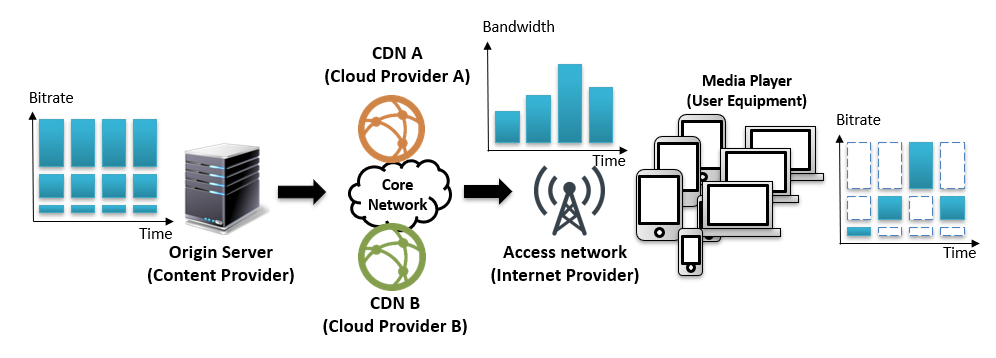
\includegraphics[width=0.8\textwidth,clip,keepaspectratio]{HAS.PNG}
	\caption{HAS-based media streaming principle}
	\label{fig:IEEECOMSThas}
	\vspace{-0.5cm}
\end{figure}

Apart from transport-layer protocols such as RTP, there are also application-layer protocols that are employed in media streaming. Table \ref{tab:IEEECOMSTalternatives} summarizes different aspects of interest when identifying the best protocol candidates to be used when streaming videos. RTP and Real Time Streaming Protocol (RTSP) \cite{schulzrinne1998real} perform low latency communications compatible with multicast media streaming. TCP-based Real-time Messaging Protocol (RTMP) \cite{thornburgh2014adobe} enables higher reliability compared to RTSP, but at the cost of having higher latency. Secure Reliable Transport (SRT) \cite{srt2021} simplifies the delivery by enabling both push and pull modes of operation. Web Real-Time Communication (WebRTC) \cite{holmberg2015web} enables media streaming through a web browser by exploiting Session Traversal Utilities for NAT (STUN) \cite{wing2008session} and Traversal Using Relays around NAT (TURN) \cite{mahy2010traversal} protocols provided by third party servers. Both SRT and WebRTC increase the security by including mandatory encryption support, while this is not always required for RTMP.
% WebRTC also adds mandatory encryption support by using Datagram Transport Layer Security (DTLS) extension which establishes the encryption keys for the Secure Real-time Transport Protocol (SRTP) employed to transfer the video stream.
HTTP Live Streaming (HLS) \cite{hls2017} and Dynamic Adaptive Streaming over HTTP (DASH) \cite{sodagar2011mpeg} increase latency due to an internal buffering to overcome network dynamics. In any case, violations on delivery timing could cause stalls and image freezes during the playback if the internal buffer gets empty. To minimise such issues, HAS allows dynamic adaptation mechanisms to track the variability of the network and select appropriate bitrate. Thus, sudden networking problems are prevented by an alternative bitrate selection from the manifest. Common Media Application Format (CMAF) \cite{hughes2017information} was a proposal to merge major streaming formats around HLS and DASH. Moreover, its Low Latency mode (LL CMAF) aims to reduce the latency by enabling HTTP chunked/push mode. Thus, the latency can be reduced and get closer to UDP-based streaming technologies. In practice, CMAF did not achieve to integration of HLS and DASH streaming formats since the implementations of Low Latency HLS (\hbox{LL-HLS}) \cite{durak2020evaluating} and Low Latency DASH (\hbox{LL-DASH}) \cite{bouzakaria2014overhead} still present some differences. Thus, \hbox{LL-HLS} and \hbox{LL-DASH} employ different approaches for HTTP transport and encryption schemes. For instance, a common feature to most HTTP-based solutions is the security by design where different encryption standards protect communications, such as Advanced Encryption Standard (AES) \cite{chown2002advanced} with Cipher Block Chaining (AES-128 CBC) or Counter mode (AES-128 CTR).

Finally, even if most existing media streaming solutions employ UDP and/or TCP, some of them, such as DASH \cite{Bhat2017} and WebRTC \cite{W3CQuic}, are already evolving and/or being tested with QUIC, a new transport protocol which is expected to substitute TCP when HTTP/3 will replace the current HTTP/2. QUIC lays on top of UDP to provide reduced latency, but with a connection control mechanism to guarantee the same reliability as TCP \cite{Quic}. There are also proposals to use HAS-based media streaming with protocols such as Stream Control Transmission Protocol (SCTP) \cite{ong2002introduction} and Multipath TCP (MPTCP) \cite{ford2011architectural}, which support multihoming, very important in recent heterogeneous network environments. Noteworthy is that MPTCP is backward compatible with the vanilla TCP, which is very useful for service deployment. Finally, efforts are already being made to develop a multipath QUIC \cite{mp-quic} protocol to combine the benefits of these approaches, but so far no HAS-based media delivery solution has used it.


\subsection{Taxonomy of Virtual Network Functions for Media Streaming}
\label{sec:IEEECOMSTtaxonomy}

\begin{figure}[htp]
	\centering
	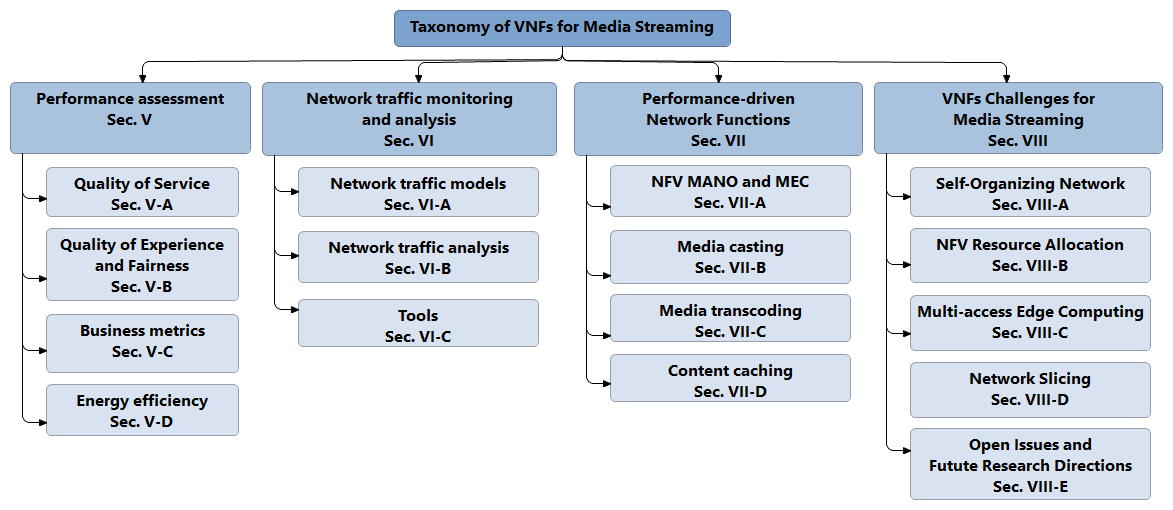
\includegraphics[width=1\textwidth,clip,keepaspectratio]{Taxonomy.png}
	\vspace{-0.3cm}
	\caption{Taxonomy of VNFs for media streaming.}
	\label{fig:IEEECOMSTcomponents}
	\vspace{-0.5cm}
\end{figure}

Following the discussion of media streaming solutions, this section reviews the motivations for the applicability of VNFs to improve the media streaming process. The taxonomy of VNFs applied to media streaming is shown in Figure \ref{fig:IEEECOMSTcomponents}.

Media streaming can leverage VNFs to enable higher network capacity and stability, media traffic optimization and other performance-related advantages. The final aim is to increase the performances of media streaming, including efficient use of network resources and end device capabilities \cite{Evensen2014} during their involvement in the streaming service. Media streaming performance indicators include Quality of Service (QoS), Quality of Experience (QoE) and Fairness, Business metrics and Energy Efficiency and illustrated in Figure \ref{fig:IEEECOMSTperformance}. We will discuss media streaming performance assessment from these different perspectives in section \ref{sec:IEEECOMSTmetrics}.

The employment of VNFs in media streaming is growing in the last few years, as the attention increases on media distribution over the newly deployed 5G networks \cite{Keltsch2018}. VNFs are intrinsically designed to follow the principles of modularity, interoperability, scalability and flexibility. However, to use VNFs more effectively in media streaming, knowledge of the network is essential. Characterizing and modelling network behavior, as well as monitoring and analyzing its traffic provide useful information to be exploited while designing, deploying a VNF \cite{Jahromi2018, Dieye2018} and managing its life-cycle \cite{alvarez_edge--cloud_2019}. Study of networks and traffic can be tackled from different points of view, as shown in Figure \ref{fig:IEEECOMSTnetwork}. There is a wide agreement that real world knowledge allows to design a more mature VNF \cite{zhang2019towards}. This knowledge is collected from network monitoring and data analysis. Considerations on network traffic monitoring and analysis are included in section \ref{sec:IEEECOMSTtraffic}.

Based on the achievements in performance assessment and knowledge acquired in network and traffic characterization, several network solutions to enable a performance-driven management of the resources are already being employed and/or investigated, as shown in Figure \ref{fig:IEEECOMSTnetfunctions}. Section \ref{sec:IEEECOMSTfunctions} deals with performance-driven network functions, including a review of the solutions provided in literature.

Finally, in the current deployment of 5G networks the VNFs have a significant role, as 5G aims to having a fully virtualized network deployment. However, there are still several open issues and challenges that need to be address in the future, as shown in Figure \ref{fig:IEEECOMSTchallenges}. Section \ref{sec:IEEECOMSTchallenges} discusses the future of VNFs in order to enable an improved media streaming process and enhanced user experience.

\subsection{Performance Assessment}
\label{sec:IEEECOMSTmetrics}

This section presents an overview of performance assessment avenues in the context of VNF-based media streaming. It involves performance aspects from multiple viewpoints, including QoS, QoE and fairness, business metrics and energy efficiency, as illustrated in Figure \ref{fig:IEEECOMSTperformance}.

\begin{figure}[htp]
	\centering
	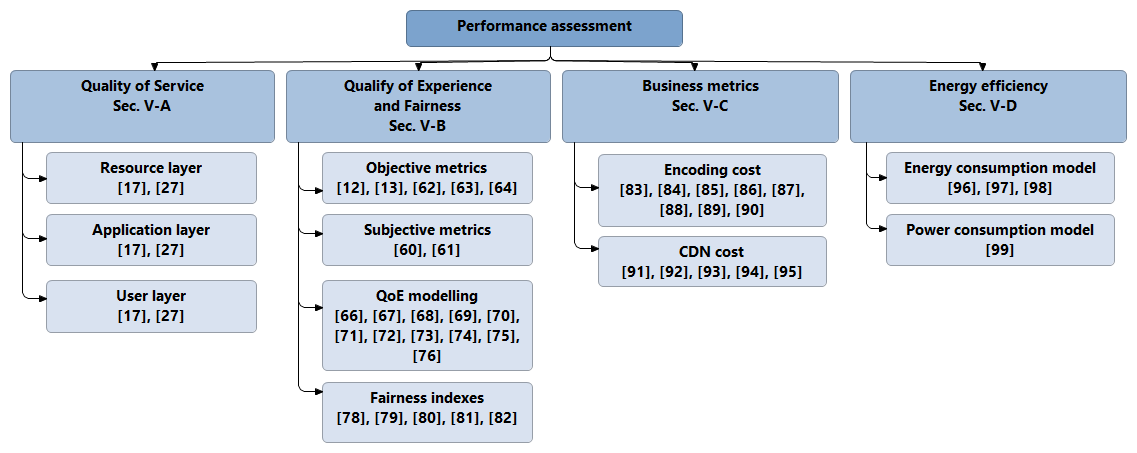
\includegraphics[width=1\textwidth,clip,keepaspectratio]{metrics.png}
	\vspace{-0.6cm}
	\caption{Multi-dimensional performance assessment.}
	\label{fig:IEEECOMSTperformance}
	\vspace{-0.6cm}
\end{figure}

\subsubsection{Quality of Service (QoS)}
\label{sec:IEEECOMSTqos}

\begin{table}[htp]
	\caption{QoS performance metrics.}
	\centering
	\label{tab:IEEECOMSTqosmetrics}
	\def\arraystretch{1.2}%  1 is the default, change whatever you need
	\setlength\tabcolsep{2.0pt} % default value: 6pt
	{\scriptsize
		\begin{tabular}{>{\centering\arraybackslash}m{\dimexpr0.15\textwidth-2\tabcolsep-\arrayrulewidth\relax}
				>{\centering\arraybackslash}m{\dimexpr0.15\textwidth-2\tabcolsep-\arrayrulewidth\relax}
				>{\centering\arraybackslash}m{\dimexpr0.3\textwidth-2\tabcolsep-\arrayrulewidth\relax}
				>{\centering\arraybackslash}m{\dimexpr0.4\textwidth-2\tabcolsep-\arrayrulewidth\relax}
		}
		\toprule
		\textbf{QoS Layer} & \textbf{Property / Category} & \textbf{Parameter / Metric} & \textbf{Description} \\
		\midrule
		\midrule
		Resource & Timeliness & Packet delay & Time taken to deliver a packet \\
		\cline{3-4}
		layer & & Packet jitter & Delay inconsistency between each packet \\
		\cline{2-4}
		& Capacity & Channel bandwidth & Occupied frequency range \\
		\cline{3-4}
		& & SNR & Signal-to-Noise Ratio\\
		\cline{3-4}
		& & PSNR & Peak Signal-to-Noise Ratio \\
		\cline{3-4}
		& & MCS & Modulation and Coding Scheme \\
		\cline{3-4} 
		& & Network bandwidth & Maximum (theoretical) data transfer rate \\
		\cline{3-4}
		& & Throughput & Effective data transfer rate \\
		\cline{2-4}
		& Reliability & BER & Bit Error Rate \\
		\cline{3-4}
		& & PLR & Packet Loss Rate \\
		\cline{3-4}
		& & Outage probability & Probability that data transfer rate is less than the required threshold \\
		\hline
		Application & Timeliness & Startup delay & Time to receive and display the first video frame \\
		\cline{3-4}
		layer & & End-to-End Delay & Time elapsed from content production to its consumption \\
		\cline{3-4}
		& & Queuing Delay & Time the video frame waits in the playback queue before being displayed \\
		\cline{3-4}
		& & Audio\&Video synchronization & Audio and video are synchronized (no lip sink error) \\
		\cline{2-4}
		& Capacity & Audio bandwidth & Audio frequency range \\
		\cline{3-4}
		& & Audio sampling rate & Audio samples recorded every second \\
		\cline{3-4}
		& & Video resolution & Pixels in each dimension that can be displayed \\
		\cline{3-4}
		& & Video frame rate & Video frames recorded every second \\
		\cline{3-4}
		& & Audio\&Video codecs & Codecs employed for audio and video encoding \\
		\cline{3-4}
		& & Audio\&Video encoding bitrates & Bitrates employed for audio and video encoding with the given codecs \\
		\cline{3-4}
		& & Audio\&Video representations & The representation levels presented in HAS \\
		\cline{2-4}
		& Reliability & Video Frame Loss & Video frames lost while displaying \\
		\cline{3-4}
		& & Representation switches & Switches between audio and/or video representation levels \\
		\cline{3-4}
		& & Stalling ratio & Probability of stalling events \\
		\cline{3-4}
		& & Stalling duration & Duration of stalling events \\
		\hline
		User & Technical & Device type & Smartphone, tablet, TV, etc. \\
		\cline{3-4}
		layer & & Screen/window size & Size of output screen/window \\
		\cline{3-4}
		& & Content type & Video conferencing (real-time), Live Streaming, Video on Demand, etc. \\
		\cline{2-4}
		& Economic & Pricing model & Flat-Rate or Pay-per-Use pricing \\
		\cline{3-4}
		& & Range of price & High, medium or low price \\
		\bottomrule
		\bottomrule
	\end{tabular}
	}
\end{table}

QoS is related to features which describe the status of network communications and/or the service supported by the network.

%application relying on networking. 
QoS properties should be physical and measurable. They are objective performance factors not affected by user's perception of the application, but they will definitely influence this perception. Due to the heterogeneity of networks and/or applications, there is not a unique set of widely accepted QoS properties. Different textbooks and publications introduce differently QoS, but in most cases they focus on a specific network and/or application context. When dealing with a network, QoS assessment consists of measuring network performance, e.g., \textit{network bandwidth}, \textit{packet loss} and \textit{latency}. When considering a particular network application, QoS is linked to a wide range of properties %, as different aspects and/or characteristics are considered,
including performance, responsiveness, availability, reliability, and application-related aspects. Each QoS property will be associated to a performance metric. Each metric will facilitate monitoring and characterization of the application property in order to understand the application behavior from that perspective. Furthermore, having a characterization of the application based on metrics associated with different QoS properties allows to put in place actions to optimize the operations of the application at run-time.

Focusing on media streaming and based on the proposals made in \cite{Jin2004} and \cite{Akhtar2017}, QoS properties are classified depending on the level of abstraction from the underlying network and hardware/software capabilities. Three main groups of QoS properties (i.e. introducing a QoS layer structure) are defined in relation to different concerns: resources, applications and users. Typical QoS properties and parameters/metrics to measure each property for each these three groups are summarized in Table \ref{tab:IEEECOMSTqosmetrics} and are discussed next.

The performance metrics at resource QoS layer quantify physical resource properties and are highly dependent on the hardware and platform employed. At this QoS layer, the most interesting ones for media streaming are \textit{timeliness}, \textit{capacity} and \textit{reliability}. Properties at resource layer should fit the requirements needed by the streaming service exploiting those resources. Metrics are %unique as they are 
not dependent on any particular application and/or user, %and their requirements are and may change depending on specific streaming service, 
rather than on the service requirements e.g., video conferencing has tight packet delay and jitter requirements, while video on demand (VOD) requires high throughput. Consequently, the performance metrics are generic for a range of applications and are measured on different OSI network model layers ranging from layer 1 (physical layer) to layer 4 (transport layer). Performance metrics at different OSI layers can characterize the same QoS property, but the abstraction from the physical resource becomes higher as the layer level increases.

At application QoS layer, similar properties to resource layer can be
%characterize 
identified, but the metrics are now completely independent from the hardware and platform, as they are application-specific and can be mapped on the network application layer (OSI layer 7). For instance the performance metrics for media streaming at application layer are highly dependent on the video and audio encoding/decoding, streaming technology for the delivery and any other application-level media processing. These metrics are completely abstracted from the network protocols, meaning that they could remain valid even if the content is a file stored locally, as the application layer is agnostic about the origin of the content (local repository or remote server). The content production itself already provides QoS parameters, via audio and video codecs and their encoding bitrates. These parameters are fixed in the encoding and/or decoding process, and they do not depend on the underlying layers. These QoS attributes refer to the characteristics of the encoding at media server and multimedia capabilities at the player device. These content and device characteristics have fixed values during the streaming session and are easily known. %, then it is enough to know media server and client capabilities in order to know these values. 
In some situations, content characteristics are not enough to describe the QoS at application layer. %Other characteristics are used in order to represent the actual QoS provided at application layer by the employed streaming service. 
Additional characteristics dependent on measurements at player side while presenting the content are used. Video impairments provide an objective measurement of the QoS level of the streaming.

Although application layer QoS properties provide high level objective metrics, they are not enough to describe user's point of view. User can be influenced by both objective and subjective factors. User layer QoS aims to identify objective metrics which describe the streaming service from user's point of view. The fact that they remain objective means that they can be measured. Here, these objective properties are completely different since they are neither based on physical resources, nor technological assets, while they deal with external features. We consider that there are two main categories to classify user layer performance metrics: technical metrics and economic ones. Technical metrics describe user device and streaming content. Economic metrics includes consideration on streaming service pricing.

Finally, user subjective metrics are instead not uniquely quantifiable as the user QoS layer ones. They are also referred to as QoE since they are focused on how the user perceives the media service. A more detailed explanation on QoE assessment is described in the next section.

\subsubsection{Quality of Experience and Fairness}
\label{sec:IEEECOMSTqoe}

\begin{table}[htp]
	\caption{QoE subjective metrics.}
	\centering
	\label{tab:IEEECOMSTqoefactors}
	\def\arraystretch{1.2}%  1 is the default, change whatever you need
	\setlength\tabcolsep{2.0pt} % default value: 6pt
	{\scriptsize
		\begin{tabular}{>{\centering\arraybackslash}m{\dimexpr0.15\textwidth-2\tabcolsep-\arrayrulewidth\relax}
				>{\centering\arraybackslash}m{\dimexpr0.15\textwidth-2\tabcolsep-\arrayrulewidth\relax}
				>{\centering\arraybackslash}m{\dimexpr0.3\textwidth-2\tabcolsep-\arrayrulewidth\relax}
		}
		\toprule
		\textbf{Category} & \textbf{Examples} & \textbf{Description} \\
		\midrule
		\midrule
		Contextual & Location & Home, office, car, etc. \\
		\cline{2-3}
		factors & Environmental characteristics & Noisy or quite, crowded or uncrowded, etc. \\
		\cline{2-3}
		& Motion & Sitting or moving, speed, etc. \\
		\cline{2-3}
		& Time & Time of the day \\
		\hline
		Human & Age & User's age \\
		\cline{2-3}
		factors & Mood & Emotional state at any time \\
		\cline{2-3}
		& Attention level & Attention level at any time \\
		\cline{2-3}
		& Goal & User's aim \\
		\cline{2-3}
		& Motivation & Level of motivation \\
		\bottomrule
		\bottomrule
	\end{tabular}
	}
\end{table}

\begin{table}[htp]
	\caption{Mean Opinion Score levels.}
	\centering
	\label{tab:IEEECOMSTmos}
	\def\arraystretch{1.2}%  1 is the default, change whatever you need
	\setlength\tabcolsep{2.0pt} % default value: 6pt
	{\scriptsize
		\begin{tabular}{>{\centering\arraybackslash}m{\dimexpr0.1\textwidth-2\tabcolsep-\arrayrulewidth\relax}
			>{\centering\arraybackslash}m{\dimexpr0.1\textwidth-2\tabcolsep-\arrayrulewidth\relax}
			>{\centering\arraybackslash}m{\dimexpr0.25\textwidth-2\tabcolsep-\arrayrulewidth\relax}
		}
		\toprule
		\textbf{MOS} & \textbf{Quality} & \textbf{Impairments} \\
		\midrule
		\midrule
		5 & Excellent & Imperceptible \\
		4 & Good & Perceptible but not annoying \\
		3 & Fair & Slightly annoying \\
		2 & Poor & Annoying \\
		1 & Bad & Very annoying \\
		\bottomrule
		\bottomrule
	\end{tabular}
	}
\end{table}

%\subsubsubsection{Quality of Experience (QoE)}
\textbf{Quality of Experience (QoE):}
QoS performance metrics do not express well users' perceived quality and satisfaction with services. A major reason relies on the fact that human evaluation is influenced by subjective factors that cannot be easily defined by quantifiable parameters and then measured. Therefore, the term QoE is employed to define and describe how a user perceives the media streaming service.
% QoS and QoE are related each other \cite{Kim2010, Alreshoodi2013} and higher QoS metric values typically lead to higher perceived quality. Anyway,
Having good values for QoS metrics is not enough to guarantee a certain level of QoE, as it does necessarily imply that the perceived quality is also good. QoS performance metrics can be considered as QoE objective metrics, but additional QoE subjective metrics are necessary. Table \ref{tab:IEEECOMSTqoefactors} shows widely used QoE subjective metrics.

The International Telecommunication Union (ITU) defines the Mean Opinion Score (MOS) \cite{Itu2016} as the measure for the QoE evaluation. It is a widely consolidated way to evaluate the QoE and consists in five quality increasing levels: 1-Bad, 2-Poor, 3-Fair, 4-Good, 5-Excellent. MOS levels are shown in Table \ref{tab:IEEECOMSTmos}. MOS level achieved by a particular streaming service is assessed by arithmetic mean over all the individual ratings by subjects which take part in the evaluation test. Nevertheless, due to the unpredictability of the subjective factors, a considerable number of scenarios could be possible while assessing the QoE. Then, ITU addresses this issue by attempting to standardize the scenario and environmental variables where the QoE ratings are collected. ITU describes the procedures to assess MOS in the correct way \cite{Itu2016-2}. The procedure intrinsically entails a long time since it requires to select a diverse group of people to represent a good approximation of a typical human audience for a given content. Then, the content should be shown to all the subjects of the chosen set and rated by them.

To simplify QoE assessment, the correlation between QoS and QoE is widely investigated in literature \cite{Kim2010, Alreshoodi2013} to profile the subjective human perception of the quality. Consequently, quality assessment based on Peak \hbox{Signal-to-Noise} Ratio (PSNR) when considering comparatively the viewed video frames and the original ones has been replaced by more accurate metrics, such as Structural similarity (SSIM) \cite{Wang2004}, SSIMplus \cite{Rehman2015}, and Netflix' Video Multi-Method Assessment Fusion (VMAF) \cite{vmaf2016}. While PSNR and SSIM are limited to spatial analysis of video frames, SSIMplus and VMAF include both spatial and temporal analysis. VMAF also moves from employing statistical analysis methods to machine-learning algorithms. VMAF evaluates several elementary metrics which measure content characteristics, type of artifacts and degree of distortion and uses inference to deliver a more accurate final score. Furthermore, Netflix introduced the concept of Per-Title Encoding \cite{PerTitle2015}, the same metrics employed to evaluate the user's QoE can be exploited at the server-side while encoding the content. Per-Title encoding allows to select the encoding bitrate which maximizes the user's QoE depending on the type of the media content (i.e. news, sport, action movie, etc.).

\begin{table}[htp]
	\caption{QoE models for HAS.}
	\centering
	\label{tab:IEEECOMSTqoemodels}
	\def\arraystretch{1.2}%  1 is the default, change whatever you need
	\setlength\tabcolsep{2.0pt} % default value: 6pt
	{\scriptsize
		\begin{tabular}{>{\centering\arraybackslash}m{\dimexpr0.3\textwidth-2\tabcolsep-\arrayrulewidth\relax}
				>{\centering\arraybackslash}m{\dimexpr0.5\textwidth-2\tabcolsep-\arrayrulewidth\relax}
				>{\centering\arraybackslash}m{\dimexpr0.1\textwidth-2\tabcolsep-\arrayrulewidth\relax}
				>{\centering\arraybackslash}m{\dimexpr0.1\textwidth-2\tabcolsep-\arrayrulewidth\relax}
		}
		\toprule
		\textbf{Model} & \textbf{Description} & \textbf{MOS scale} & \textbf{Year} \\
		\midrule
		\midrule
		De Vriendt et al. \cite{DeVriendt2013} & Bitrate model, PSNR/SSIM model, chunk-MOS model and Quality level model & yes & 2013 \\
		Yin et al. \cite{Yin2014} & Normalized QoE & no & 2014 \\
		Xue et al. \cite{Xue2014} & Instantaneous and cumulative QoE with exponential decay & no & 2014 \\
		DASH-UE (Liu et al.) \cite{Liu2015} & DASH User Experience model & no & 2015 \\
		Bentaleb et al. \cite{Bentaleb2016} & SSIMplus-based QoE & yes & 2016 \\
		SQI (Duanmu et al.) \cite{Duanmu2016} & Streaming QoE Index & yes & 2016 \\
		U-vMOS (Huawei) \cite{Huawei2016} & User/Unified/Ubiquitous video Mean Opinion Score & yes & 2016 \\
		ITU-T P.1203 \cite{itup1203} & Parametric bitstream-based quality assessment for HAS services & yes & 2017 \\
		KSQI (Duanmu et al.) \cite{Duanmu2019} & Knowledge-driven streaming quality index & yes & 2019 \\
		De Fez et al. \cite{deFez2020} & Modified Yin\cite{Yin2014}-model, PSNR-based model, VMAF-based model & yes/no & 2020 \\
		ITU-T P.1204 \cite{itup1204} & Bitstream-based/pixel-based/hybrid models for resolutions up to 4K & yes & 2020 \\
		\bottomrule
		\bottomrule
	\end{tabular}
	}
\end{table}

Focusing on HAS, diverse metrics have been considered to create QoE models based on its characteristics.
QoE models span from pixel-level comparison between received frames and original ones (e.g. PSNR, SSIM, SSIMplus and VMAF) to \hbox{content-agnostic} models with sophisticated equations which consider a wide range of parameters, including available representation bitrates, frequency of bitrate changes and buffering duration.
By focusing on objective metrics only, there is an inevitable loss of accuracy, but it has several practical advantages. The absence of human feedback on the QoE reduces the test time and result processing can be automated to be carried out online. Common QoE models are presented in Table \ref{tab:IEEECOMSTqoemodels}. Even ITU defines MOS as the standard metric, MOS scale is not employed by all the QoE models as a measure of achieved QoE ratings.

ITU proposes several models, including ITU-T P.1203 \cite{itup1203} and ITU-T P.1204 \cite{itup1204}. ITU-T P.1203 \cite{itup1203} is a parametric bitstream-based model for HAS services which expresses the result in terms of MOS. The model considers both audio and video features, the impact of buffering on perceived quality and also takes into account information on the employed display device. Due to the performed bitstream analysis, a real implementation \cite{Robitza2018} of this model is computationally intensive as content is analyzed on a per media segment and per video frame basis. The model introduces four modes of operation, from 0 to 3,  to tune the trade-off between accuracy and complexity. Lower modes are less accurate to reduce complexity, while higher mode increase the complexity to gain accuracy. Finally, modes 3 and 4 also raise security issues, as the bitstream must be unencrypted/decrypted to access the required input information. ITU-T P.1204 \cite{itup1204} the newest standard from ITU and it is not actually a unique model, but it groups models of different type: bitstream-based, pixel-based and hybrid models. ITU-T P.1204 is meant to be an extension to ITU-T P.1203, as it is focused on higher resolutions (up to 4K). Unfortunately, both ITU models show intrinsic computational complexity.

As an alternative to the complex ITU models, other QoE models are proposed in the literature. In equation (\ref{eq:IEEECOMST2021mosp}) De Vriendt et al. \cite{DeVriendt2013} formulate a general expression for QoE models to predict the results of HAS services on MOS scale.

\begin{equation}
	\label{eq:IEEECOMST2021mosp}
	M_{pred} = \alpha*\mu - \beta*\sigma - \gamma*\phi + \delta
\end{equation}
where $\alpha$, $\beta$, $\gamma$ $\delta$ are tunable coefficients. $\mu$ and $\sigma$ are average of the quality of the displayed HAS representations and its standard deviation, respectively. Finally, $\phi$ takes into account both average duration and frequency of freeze events. From the equation, it is clear that the quality estimation is influenced by some major factors of HAS services: quality associated to each representation, switches between representations and stalling/buffering events. The coefficients are tuned by minimizing the Mean Square Error (MSE) between the predicted MOS values (M$_{pred}$) and the real ones assessed by rating a set of different video clips on different devices, as shown is equation (\ref{eq:IEEECOMST2021mosmse}).

\begin{equation}
	\label{eq:IEEECOMST2021mosmse}
	\frac{\sum\limits_{n=1}^{N} (M_{pred,n} - MOS_n)^2}{N}
\end{equation}

The selection of values for $\mu$ and $\sigma$ leads to different types of models, as several ways to define the quality of a representation are possible. De Vriendt et al. \cite{DeVriendt2013} state that there are at least 4 ways to select the quality:

\begin{itemize}
	\item Bitrate model: the quality is defined by the bitrate of the representation.
	\item PSNR or SSIM model: the quality is defined by the average PSNR or SSIM over all the frames of a segment.
	\item Chunk-MOS model: the quality is not calculated from the representation, but it is part of the same MSE minimization process.
	\item Quality level model: the quality levels are equally spaced between a minimum and a maximum value.
\end{itemize}
The authors conclude that the chunk-MOS model has the best performance, with more flexibility for optimization since two more parameters ($\mu$ and $\sigma$) are varied to improve the model.

Yin et al. \cite{Yin2014} suggest a similar approach that considers the same variables to assess a normalized QoE. Later models start from a similar optimization problem expressed by the equation (\ref{eq:IEEECOMST2021mosp}) and aim to expand by including further variables or defining differently the quality associated to each representation. Liu et al.'s DASH-UE \cite{Liu2015}, SQI (Duanmu et al.) \cite{Duanmu2016} and Huawei's User/Unified/Ubiquitous video MOS (UvMOS) \cite{Huawei2016} also include the startup (initial) delay in the equation. They assert that startup delay has negative effects on the user's QoE. Xue et al. \cite{Xue2014} perform instantaneous QoE score estimations and introduce an exponential decay to emulate the forgetting curve of human perception when evaluating the cumulative QoE score.

Bentaleb et al. \cite{Bentaleb2016} employ SSIMplus \cite{Rehman2015} to assess the quality related to each representation instead of the four approaches proposed by De Vriendt et al. \cite{DeVriendt2013}. Duanmu et al.'s Knowledge-driven Streaming Quality Index (KSQI) \cite{Duanmu2019} considers the same variables, aims to include a human visual system (HVS) analysis result to improve QoE modelling. The authors derive a system of linear inequalities from QoE subjective studies which allows to improve the optimization problem of QoE modelling.

Finally, De Fez et al. \cite{deFez2020} propose three different models. The first one is a modified Yin et al. \cite{Yin2014} model which improves accuracy by using the actual video segment bitrate instead of the average value of the segment representation. The second and the third ones are a PSNR-based model and a VMAF\cite{vmaf2016}-based model, respectively. These models employ PSNR and VMAF metrics to evaluate the quality of each segment instead of the actual video bitrate.

%\subsubsubsection{Fairness}
\textbf{Fairness:}
While the number and diversity of approaches to assess QoE is large, there are very few metrics to measure fairness. Jain's fairness index \cite{jain1984quantitative} is one of the most widely used such metric and was originally introduced to express the fairness of throughput distribution across multiple flows that share a common distribution infrastructure. However, its applicability can be extended to any set of values $x_i$, which are measured on a scale, where $i=\overline{1,N}$. Note that the minimum Jain's fairness value is $\frac{1}{N}$ and the maximum is 1.

\begin{equation}
	\label{eq:IEEECOMST2021Jain}
	J(x_1, x_2, ... x_N)=\frac{({\sum_{i=1}^{N}x_{i}})^2}{\sum_{i=1}^{N}{x_{i}}^2}
\end{equation}

Unfortunately, even though many networking parameters can be measured on ratio scales, there are some (i.e., QoE is among them), which are expressed on interval scales, such as the 5-point MOS scale, for instance. For one of these situations, Ho{\ss}feld et al. \cite{Hossfeld2016} have proposed a QoE Fairness index based on the lowest $L$ and highest $H$ bounds of the rating scale. In (\ref{eq:IEEECOMST2021Hossfeld}) $\sigma$ is the standard deviation and measures the degree of dispersion of the values. Ho{\ss}feld's fairness index has values in the interval $[0,1]$, where 0 is associated with total unfairness and 1 with perfect fairness.

\begin{equation}
	\label{eq:IEEECOMST2021Hossfeld}
	F=1-\frac{2\sigma}{H-L}
\end{equation}

There are some situations when classic fairness metrics do not reflect well the actual distribution of values. A more generic product-based fairness metric, presented in equation (\ref{eq:IEEECOMST2021Product}), was discussed in \cite{Shi2014} along with other fairness metrics. In equation (\ref{eq:IEEECOMST2021Product}) $f$ is a transformation function which can be defined according to the desired effect, allowing for very high flexibility in the fairness assessment.

\begin{equation}
	\label{eq:IEEECOMST2021Product}
	\mathcal {P}(x)=\prod _{i=0}^{N}f\left({\frac {x_{i}}{\max(x)}}\right)
\end{equation}

The simplest product-based fairness index which uses a linear function $f(x)=x$ is represented in equation (\ref{eq:IEEECOMST2021linProd}).

\begin{equation}
	\label{eq:IEEECOMST2021linProd}
	LP(x)=\frac{\prod _{i=0}^{N}x_{i}}{\max(x)^{N}}
\end{equation}

Two other product-based fairness indexes, G's and Bossaer's, are defined using $f(x)=\sin(x\pi /2)^{\frac {1}{k}}$ and $f(x)=x^{\frac {1}{k}}$, respectively. While the first emphasizes the values closer to $\max(x)$, the later inflates the values closer to 0.

Other approaches include the general fairness model proposed by Lan et al. \cite{Lan2010} and min-max and max-min-based fairness indexes introduced by Radunovic et al. \cite{Radunovic2007}.

\subsubsection{Business Metrics}
\label{sec:IEEECOMSTbusiness}

\begin{table}[t]
	\caption{Business costs for media streaming.}
	\centering
	\label{tab:IEEECOMSTcosts}
	\def\arraystretch{1.2}%  1 is the default, change whatever you need
	\setlength\tabcolsep{2.0pt} % default value: 6pt
	{\scriptsize
	\begin{tabular}{>{\centering\arraybackslash}m{\dimexpr0.25\textwidth-2\tabcolsep-\arrayrulewidth\relax}
			>{\centering\arraybackslash}m{\dimexpr0.25\textwidth-2\tabcolsep-\arrayrulewidth\relax}
			>{\centering\arraybackslash}m{\dimexpr0.3\textwidth-2\tabcolsep-\arrayrulewidth\relax}
		}
		\toprule
		\textbf{Category} & \textbf{Examples} & \textbf{Description} \\
		\midrule
		\midrule
		Capital expenditure & Buildings and furniture & Buy buildings, server racks, etc. \\
		\cline{2-3}
		& Equipment & Servers, laptops, monitors, etc. \\
		\cline{2-3}
		& Intangible assets & Purchased licenses or patents \\
		\cline{2-3}
		& Software & Commercial proprietary software \\
		\hline
		Operational & Utilities & Electricity, water, etc. \\
		\cline{2-3}
		expenditure & Employees & Salaries and benefits \\
		\cline{2-3}
		& Research and development & Develop/improve media service \\
		\cline{2-3}
		& Encoding & Costs due to content preparation \\
		\cline{2-3}
		& CDN usage & Costs due to content delivery \\
		\bottomrule
		\bottomrule
	\end{tabular}
	}
\end{table}

Achieving higher QoS and QoE values comes at a cost for the Content Provider (CP), because there are generally increased expenses in terms of network/services resources. %to increase them. 
%Having higher resources means higher costs. 
Nevertheless, CP's strategies should focus on minimizing the business costs, while guaranteeing the same or even higher QoS/QoE. Table \ref{tab:IEEECOMSTcosts} provides a list of common business costs for a typical CP-based media streaming.

Capital Expenditure (CAPEX) refers to expenses incurred by the CP for the acquisition or improvement of fixed assets that are necessary for the business. CAPEX includes intangible assets, specific software as well as expenses related to licenses and patents payments. In this sense, the use of video codecs is the most evident example. Moving Picture Experts Group (MPEG) codecs require payments of licenses (royalties) for commercial use. H264 remains widely used, and it is still supported by most end devices. The royalties for using HEVC have increased \cite{OzerLicense} and this fact prevents some CPs from using HEVC (and maybe its successor VVC) and drives their interest towards royalty-free alternatives \cite{OzerLicense-2}. VP8 and VP9 were developed and released by Google, which later joined the Alliance for Open Media (AOM) with other mayor tech companies to work on the AV1 video codec. Nevertheless, as the MPEG-Google/AOM codecs struggle is still on-going, other factors may influence CP decisions on the employed codec, including limitations from device manufacturers (hardware encoding and decoding capabilities) and/or browser capabilities \cite{MozillaCodecs}.

Operational Expenditure (OPEX) refers to on-going costs for running the business and inherent to the operation of the assets. Except from expenses common with every business, encoding and CDN usage are the most relevant and specific to media streaming services. Once the codec has been chosen, the encoding operations may have other operational costs that vary depending on the encoder choice (i.e., open-source or commercial) and where the encoder runs (i.e., cloud or on-premise encoding). Cloud encoding prices are established by cloud providers \cite{OzerCloud}, while on-premise coding depends on the hardware selection and maintenance. On the other side, on-premise encoding allows to have more control on the processed data and content compared to cloud encoding \cite{BasuEncoding, PellenEncoding}. The total encoding cost is expressed in equation (\ref{eq:IEEECOMST2021enc}).
\begin{equation}
	\label{eq:IEEECOMST2021enc}
%	\begin{split}
%		Enc_{cost} = & codec_{royalties} + encoder_{price} + \\
%		& + server_{cost} + processing_{cost}
%	\end{split}
	Enc_{cost} = codec_{royalties} + encoder_{price} + server_{cost} + processing_{cost}
\end{equation}

In equation (\ref{eq:IEEECOMST2021enc}), codec$_{royalties}$ + encoder$_{price}$ expenses belong to CAPEX, while processing$_{cost}$ is an OPEX. server$_{cost}$ depends on the strategy, a cloud encoder generates an OPEX, while an on-premise encoder needs an equipment investment which is a CAPEX. Focusing on processing$_{cost}$, employing Per-Title encoding and CMAF can reduce the OPEX. Per-Title encoding enables optimization of the encoder adjustment \cite{LambeauPerTitle}, and provides a more effective bitrate and resolution choice to optimize the trade-off between QoE and processing resources. CMAF guarantees compatibility between different HAS technologies, meaning that the encoded content can be shared between them. Thus, a single encoding operation is necessary for both DASH and HLS \cite{TimmererCMAF}.

The cost of CDN resources depends on their ongoing utilization \cite{verbrugge2006}. Not all providers publish their own pricing plans since in most of the cases they offer personalized plans to each customer. Nevertheless, \cite{dacast2019}, \cite{CdnCalculator} and \cite{wowza} reveal common factors that influence the OPEX for CDN resources, such as the outbound network traffic, storage occupancy and usage time. Thus, CDN OPEX can be expressed as (\ref{eq:IEEECOMST2021opex}) \cite{Viola2020}:
\begin{equation}
	\label{eq:IEEECOMST2021opex}
%	\begin{split}
%		CDN_{cost} = & \sum_{i=1}^{N} ( \alpha_{loc_i}*Tr_i + \beta_{loc_i}*K_{req_i} + \\
%		& + \gamma_{loc_i}*T_i + \delta_{loc_i}*St_i + \epsilon_{loc_i})
%	\end{split}
	CDN_{cost} = \sum_{i=1}^{N} ( \alpha_{loc_i}*Tr_i + \beta_{loc_i}*K_{req_i} + \gamma_{loc_i}*T_i + \delta_{loc_i}*St_i + \epsilon_{loc_i})
\end{equation}

In equation (\ref{eq:IEEECOMST2021opex}), \textit{Tr$_i$} and \textit{K$_{req_i}$} represent the traffic volume and the number of HTTP requests producing this traffic. \textit{T$_i$} and \textit{St$_i$} are the utilization time for a CDN (active sessions from video players) and the employed storage at CDN, respectively. Finally, $\alpha_{loc_i}$, $\beta_{loc_i}$, $\gamma_{loc_i}$, $\delta_{loc_i}$, and $\epsilon_{loc_i}$ are multiplicative coefficients established by the CDN provider and are dependent on the location of CDN resources (the cost of a cloud server depends on the geographical location). CPs usually employ simultaneously more than one CDN to increase coverage and in consequence the addition means a sum over the \textit{N} available CDNs. The values of the coefficients depend on the business model and the pricing plan of each CDN provider. On the contrary, the variables which depend on the CDN usage (\textit{Tr$_i$}, \textit{K$_{req_i}$}, \textit{T$_i$} and \textit{St$_i$}) can be exploited by the CP to optimize the CDN resource selection and achieve a trade-off between QoS/QoE and cost.

\subsubsection{Energy Efficiency}
\label{sec:IEEECOMSTenergy}
Efficient usage of energy has become a worldwide critical challenge. There is a very strong motivation for researchers to propose and develop energy efficient techniques in order to manage the power consumption in both current and future network environments. The range of green networking solutions covers a wide area. There are centralized network-centric approaches, where operators would deploy and positively influence large scale systems. A different strategy is based on individual solutions, which can be deployed considering a user-centric paradigm. There are energy preservation solutions which target equipment functionality and others which influence data exchange protocols, mechanisms which involve single components and others which target communication and cooperation between units, solutions deployed at a single network layer or across multiple layers, schemes which are made public and approaches which are proprietary, etc.

In this complex energy-aware research, 
%development and deployment space and in the context of this paper,
there is a natural interest on solutions for energy efficient delivery of multimedia content with focus on end-user terminal devices. The latest wireless smart mobile devices are deployed with limited battery-based power resources, while computational and content presentation-related complexity has increased exponentially. 
Kennedy et al. \cite{kennedy2013} studied mobile device components' energy consumption. These authors have noted that screen, CPU, audio and network units scored the highest in terms of energy consumption, with a large gap between minimum and maximum values for the presentation components (i.e., screen and speakers). Lately, by using hardware optimization solutions for content presentation, the consumption associated to screen and audio interfaces has been reduced at the cost of increased processing complexity as well as increased data transfer.
%has reduced energy consumption for screen and audio, but content processing complexity and amount of data transferred has increased making these two energy consumption avenues very important. 
It is therefore fundamental to achieve energy efficiency for rich media content exchange between smart device and other sources or in-between such devices in order to extend operational activity of the devices and support high user QoE. 

For a device, energy consumption $E$ is the sum of the energy consumed in data transmitting mode (Tx), data receiving mode (Rx), sleeping mode (Sl) and during state transition (Sw).
%, respectively.
\begin{equation}
	\label{eq:IEEECOMST2021encons}
	\begin{split}
		E = {E_{Tx}} + {E_{Rx}} + {E_{Sl}} + {E_{Sw}}
	\end{split}
\end{equation}

Energy efficiency is generally defined as information bits per unit of transmission energy. A typical function of energy efficiency calculation for an additive white Gaussian noise channel is shown in equation (\ref{eq:IEEECOMST2021eneta})
\cite{mcclaning2000}:
\begin{equation}
	\label{eq:IEEECOMST2021eneta}
	\begin{split}
		\eta = \frac{2R}{N_0(2^{2R}-1)}
	\end{split}
\end{equation}
where the channel capacity $R$ is defined as in equation (\ref{eq:IEEECOMST2021enR}):
\begin{equation}
	\label{eq:IEEECOMST2021enR}
	\begin{split}
		R=\frac{1}{2}\log{(1+\frac{P}{N_0B})}
	\end{split}
\end{equation}
and $P$ represents the transmit power, $N_0$ represents the noise power spectral density and $B$ represents the system bandwidth.

However, most solutions require dynamic computation of energy consumption and the components with the largest contribution to the overall energy budget are $E_{Tx}$ and $E_{Rx}$. Even though transmission energy consumption is expected to exceed the ammount required by reception functions, the literature associates the energy consumption with network interfacing activity in general,  and not with any specific communication.

There are two models oftenly used in the literature.
In the context of a mobile device, equation (\ref{eq:IEEECOMST2021eneta2}), proposed by Trestian et al. in \cite{Trestian2013}, calculates the energy consumption as follows:
\begin{equation}
	\label{eq:IEEECOMST2021eneta2}
	\begin{split}
		E = t(r_t + Th*r_d)
	\end{split}
\end{equation}
where $E$ is the estimated energy consumption (Joule) for a RAN, $t$ represents the transaction time (seconds), $r_t$ is the mobile device’s energy consumption per time unit (Watt), $Th$ is the throughput (Kbps) and $r_d$ is the energy consumption rate for the data stream (Joule/Kbyte). The parameters $r_d$ and $r_t$ are device specific and differ for various network interfaces present at the device side.

A second power consumption model for a sensor node was introduced by Zou et al. in \cite{Zou2017} and is described by equation (\ref{eq:IEEECOMST2021power}). According to this model, the theoretical power consumption $p_{r}$ of a wireless interface $r$ is proportional to the throughput $Th_{r}$, as indicated in equation (\ref{eq:IEEECOMST2021power}).
\begin{equation}
	\label{eq:IEEECOMST2021power}
	p_{r}(Th_{r})=\alpha_{r}*Th_{r}+\beta_{r}+\gamma_{r}
\end{equation}

In equation (\ref{eq:IEEECOMST2021power}), $p_{r}$ is the power expressed in Watts, $\alpha_{r}$ is the energy consumption rate for data in $mJ/Kb$ for the interface $r$, $Th_{r}$ denotes the data rate in $Kbps$ on interface $r$, $\beta_{r}$ is the energy consumption per unit time in $mWatt$ for the interface $r$ and $\gamma_{r}$ is a constant which is a tunable value associated with the background energy consumption for interface $r$.
If the node is equipped with a total of $R$ interfaces, the total power consumption is calculated as in equation (\ref{eq:IEEECOMST2021totP}):
\begin{equation}
	\label{eq:IEEECOMST2021totP}
	P = \sum_{r\in R}p_{r}(Th_{r})
\end{equation}

\subsection{Network Traffic Monitoring and Analysis}
\label{sec:IEEECOMSTtraffic}

This section overviews major research activities related to network and traffic monitoring. Studies are performed from different points of view, as shown in Figure \ref{fig:IEEECOMSTperformance}. Research activities include investigations on statistical models which can approximate network traffic behavior and analysis of the network traffic to acquire valuable information to be used to improve the network performance. In this section we also include a review of tools employed for performance monitoring and network simulation.

\begin{figure}[htp]
	\centering
	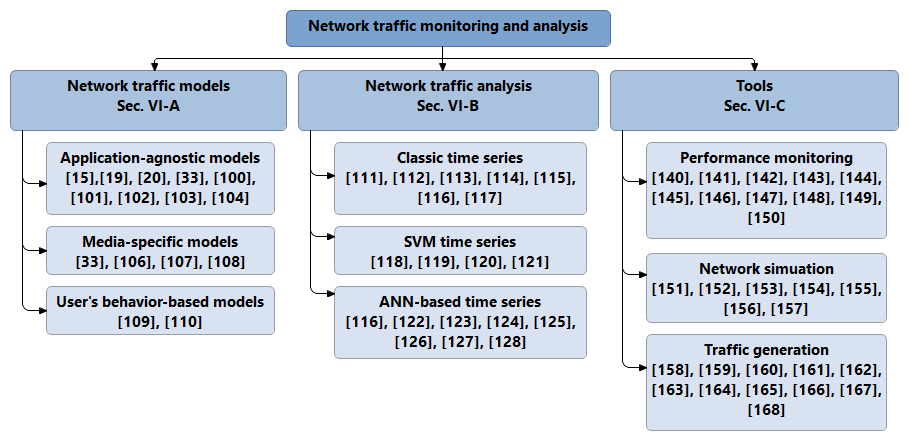
\includegraphics[width=0.75\textwidth,clip,keepaspectratio]{network.png}
	\caption{Network traffic monitoring and analysis.}
	\label{fig:IEEECOMSTnetwork}
	\vspace{-0.5cm}
\end{figure}

\subsubsection{Network Traffic Models}
\label{sec:IEEECOMSTmodels}

\begin{table}[htp]
	\caption{Application-agnostic network traffic models.}
	\centering
	\label{tab:IEEECOMSTtrafficmodels}
	\def\arraystretch{1.2}%  1 is the default, change whatever you need
	\setlength\tabcolsep{2.0pt} % default value: 6pt
	{\scriptsize
		\begin{tabular}{>{\centering\arraybackslash}m{\dimexpr0.3\textwidth-2\tabcolsep-\arrayrulewidth\relax}
			>{\centering\arraybackslash}m{\dimexpr0.7\textwidth-2\tabcolsep-\arrayrulewidth\relax}
		}
		\toprule
		\textbf{Model} & \textbf{Description} \\
		\midrule
		\midrule
		Poisson \cite{Guerin2003} & Memoryless distribution of the arrivals from independent sources (Poisson sources) \\
		Non-stationary Poisson \cite{karagiannis2004} & Non-stationary Poisson behavior at multi-second time scales \\
		Log-normal \cite{Bhattacharjee2010} & Inter-arrival times from aggregated sources modelling \\
		Pareto \cite{Bhattacharjee2010, Zhang2007} & Inter-arrival times from aggregated sources modelling, End-to-end delay modelling \\
		Weibull \cite{Arfeen2013} & Inter-arrival processes (packets, flows and sessions) modelling \\
		Markov \cite{Adas1997} & Model of activities of a traffic source with exponentially distributed time between state transitions \\
		Embedded Markov \cite{Adas1997} & Model of activities of a traffic source with arbitrary probability distributed time between state transitions \\
		\bottomrule
		\bottomrule
	\end{tabular}
	}
\end{table}

Over the years, network traffic models have been thoroughly studied within the communication networks domain to describe the behaviour of discrete entities, namely, packets, connections, etc. In statistics and probability theory, this kind of traffic is described as a Point Process \cite{Daley2007}. Many models have been proposed, with advantages and disadvantages, appropriate or not to different types of networks (i.e. Ethernet, Wi-Fi, LTE/5G, etc.) and with support for diverse scenarios. 
%Each proposed traffic model has its own pros and cons. 
The choice of traffic model to employ depends on the particular network under study and the demand characteristics. The models are useful to perform any optimization and to produce a robust and reliable network infrastructure design. Moreover, they are essential to design and experiment network services since they can be employed to recreate a realistic traffic scenario in a controlled environment (laboratory). Thus, network services are tested and validated before being deployed in production. Obviously, each model has some assumptions that limits its usage. In other words, the models are not perfect, but their approximation is good enough for experimentation purposes.

In \cite{Chandrasekaran2009} and \cite{Mohammed2011}, the most common application-agnostic network traffic models are presented, i.e., these models focus on characterizing generic network packet arrivals. The Poisson distribution model is one of the oldest models, but it is still widely employed across the literature to model packet arrivals from independent sources \cite{Guerin2003}. The authors of \cite{karagiannis2004} carried out a deep analysis of network traffic to study the limitations of the Poisson model. The authors propose a non-stationary Poisson model as the Poisson model accurately characterizes traffic only at sub-second time scales. At multi-second time scales the traffic seems to have a non-stationary behavior. The Log-normal and Pareto distributions are employed to model inter-arrival times from aggregated sources \cite{Bhattacharjee2010}. Moreover, the Pareto distribution also models end-to-end network delay \cite{Zhang2007}. The Weibull distribution describes inter-arrival processes at different levels, meaning that it fits with packets, flows and sessions arrivals by tuning its parameters \cite{Arfeen2013}. Markov and Embedded Markov models are used for network sources with a finite number of states, e.g., voice telephony has idle, busy and transmit states \cite{Adas1997}, and they differ in describing the time between state transitions. Table \ref{tab:IEEECOMSTtrafficmodels} presents the most employed application-agnostic models. 

Other studies have focused on media specific applications instead on traffic-agnostic ones. In \cite{Navarro-Ortiz2020}, the authors employ some models proposed in literature to describe the traffic generated by specific 5G use cases/applications. In \cite{Liu2009}, a traffic analysis of an IPTV CDN network is presented. The authors find that the bitrate of multicast flow is relatively stable and depends on the number of live broadcast channels, while the bitrate of a unicast flow varies along the day and presents differences between weekdays and weekend. In \cite{rao2011}, the traffic characteristics of Netflix and YouTube were analyzed, and the findings reveal that data is transferred through ON-OFF cycles, whose duration is dependent on the user's device and browser. In \cite{zink2009}, a study of YouTube traffic reveals that the traffic is highly dependent on the hour of the day. Moreover, the inter-arrival between two consecutive video requests depends on the popularity of the video.

Finally, \cite{yu2006} and \cite{Liu2014} present two studies of user behavior while accessing streaming services. In \cite{yu2006}, the authors focus on VOD streaming and they note that the user inter-arrival rate can be modelled by a modified Poisson distribution. Once streaming was accessed, the session length varied depending on the video duration. Furthermore, they find that more than half of the overall sessions end within ten minutes, while more than one third ended within 5 min. The user behavior has also some variations depending on the day of the week, as during the weekend, the video requests increase. In \cite{Liu2014}, the authors also consider live streaming. They find that a Poisson distribution is less accurate when modelling user inter-arrival for live streaming services than for VOD ones.

\subsubsection{Network Traffic Analysis}
\label{sec:IEEECOMSTanalysis}

\begin{table}[htp]
	\caption{Methods for time series analysis applied to networks.}
	\centering
	\label{tab:IEEECOMSTmodels}
	\def\arraystretch{1.2}%  1 is the default, change whatever you need
	\setlength\tabcolsep{2.0pt} % default value: 6pt
	{\scriptsize
		\begin{tabular}{>{\centering\arraybackslash}m{\dimexpr0.15\textwidth-2\tabcolsep-\arrayrulewidth\relax}
			>{\centering\arraybackslash}m{\dimexpr0.24\textwidth-2\tabcolsep-\arrayrulewidth\relax}
			>{\centering\arraybackslash}m{\dimexpr0.1\textwidth-2\tabcolsep-\arrayrulewidth\relax}
			>{\centering\arraybackslash}m{\dimexpr0.12\textwidth-2\tabcolsep-\arrayrulewidth\relax}
			>{\centering\arraybackslash}m{\dimexpr0.14\textwidth-2\tabcolsep-\arrayrulewidth\relax}
			>{\centering\arraybackslash}m{\dimexpr0.27\textwidth-2\tabcolsep-\arrayrulewidth\relax}
		}
		\toprule
		\textbf{Method} &  \textbf{References} & \textbf{Approach} & \textbf{Number of variables} & \textbf{Configuration / parameters} & \textbf{Description} \\
		\midrule
		\midrule
		ARIMA & \cite{calheiros2014, dong2015, amin2012, amin2012-2, Wang2017-2} & classic & univariate & regression, integration and moving average parameters & Autoregressive integrated moving average \\
		SETARMA & \cite{amin2012} & classic & univariate & regression, moving average and threshold delay parameters & Self-exciting threshold autoregressive moving average \\
		GARCH & \cite{amin2012} & classic & univariate & regression and lag length parameters & Generalized autoregressive conditional heteroskedastic \\
		Holt’s linear trend & \cite{dong2015} & classic & univariate & smoothing factor & Secondary or double exponential smoothing time series \\
		Holt-Winters’ seasonal & \cite{Szmit2012, Shahin2017} & classic & univariate & smoothing factor & Cubic or triple exponential smoothing time series \\
		% Wavelet transform \cite{Huang2001, Wang2002} & Wavelet-based time series & wavelet & univariate & a-priori (wavelet coefficients) \\
		SVR & \cite{Mirza2010, Bermolen2009} & SVM & multivariate & weight vector and offset & Support Vector Regression \\
		H-SVM & \cite{Feng2011} & SVM & multivariate & weight vector and offset & Hierarchical Support Vector Machine \\
		Multi-class SVM & \cite{Chen2013} & SVM & multivariate & weight vector and offset & Multi-class Support Vector Machine \\
		Feed-forward NN & \cite{zadeh2010} & ANN & multivariate & weight and bias & Feed-forward neural network \\
		MLP & \cite{Szmit2012, Khotanzad2003} & ANN & multivariate & input vector, weight vector and bias & Multi-layer Perceptron \\
		FNN & \cite{Khotanzad2003} & ANN & multivariate & input vector, weight vector and bias & Fuzzy Neural Network \\
		RNN & \cite{belhaj2009} & ANN & multivariate & input, output and forget factors & Recurrent neural network \\
		LSTM & \cite{trinh2018, Azzouni2018, martinez2021identification} & ANN & multivariate & input, output and forget factors & Long short-term memory \\
		ESN & \cite{Cui2014} & ANN & multivariate & input, reservoir and output weights & Echo State Network \\
		% Deep RL & \cite{Koo2019} & ANN & multivariate & states, actions and rewards & Deep Reinforcement Learning \\
		\bottomrule
		\bottomrule
	\end{tabular}
	}
\end{table}

The ability to model and generate realistic network scenarios offers the possibility to design and deploy network functions that adjust to the network traffic at any moment. Analyzing network traffic and applying time series analysis means a further step since it allows to forecast future network traffic. Network functions could move from reactive to proactive approach by exploiting predicted future conditions of the network. Actions are proactively taken when performances are going to not be satisfied. Thus, network under-performance and outages are prevented.

There are many methods proposed in literature for time series analysis.
Among them, we distinguish classic time series, Support Vector Machine (SVM) time series and Artificial Neural Network (ANN)-based time series \cite{Sapankevych2009}. The choice of a predictor based on one of the different time series approaches depends on the characteristics of the network and different approaches are suitable for traces from different sources \cite{Iqbal2019}. Moreover, in the same scenario different approaches could be combined to predict both long-term traffic demand and short-term network metrics \cite{Kryftis2015}.
Classic time series approaches are well known, as they were defined prior to the raise of telecommunication networks. On the contrary, SVM and ANN-based solutions can be seen as new contenders to classic ones, as Machine Learning (ML) application for time series prediction \cite{Bontempi2012} is relatively new (SVM and ANN are two different supervised learning approaches). Time series methods employed for network forecasting are shown in Table \ref{tab:IEEECOMSTmodels}. The table also presents the main differences between them, such as the number of input and output variables and the selection of internal parameters. ML (SVM and ANN) models take the advantage from the knowledge of several variables as input (multivariate), while classic ones are limited to one (univariate). The same is valid for output variables, ML models can output more than one. The outcomes of \cite{azari2019} and \cite{azari2019-2} reveal that a higher number of input variables improves the traffic predictions of a ML model (the authors employ a Long short-term memory model) when compared to a classic one (the authors employ an autoregressive integrated moving average model).

% Moreover, the selection of internal parameters is performed through a-priori evaluation for classic approaches, while ML models exploit dataset of previous collected metrics to train themselves.

The autoregressive integrated moving average (ARIMA) \cite{Hyndman2018} is one of the oldest time series method and widely employed in literature as reference method for evaluating any other time series approach. In \cite{calheiros2014}, ARIMA is employed to predict the workload of cloud services. Historical observed requests are exploited to predict the volume of requests during the next time interval. The authors find limitations to track traffic peaks accurately. In \cite{Wang2017-2}, ARIMA is instead employed to predict the request number and the amount of data traffic. Other limitations to ARIMA are found in \cite{amin2012} and \cite{amin2012-2} when modelling QoS attributes which have non-linear behaviors, i.e., time between QoS violations. Thus, they do not fit the linear assumption of ARIMA. Self-exciting threshold autoregressive moving average (SETARMA) \cite{amin2012} and generalized autoregressive conditional heteroskedastic (GARCH) \cite{amin2012-2} are integrated with ARIMA in hybrid linear and non-linear models to overcome ARIMA limitations.

Exponential smoothing \cite{Holt2004} is a subset of classic time series method. Holt's linear trend method (secondary or double exponential smoothing) is employed in \cite{dong2015}. The authors find it complementary to ARIMA when predicting throughput in an LTE network. ARIMA outperforms the exponential smoothing on weekdays, while the exponential smoothing prediction are more accurate on weekends.
Holt-Winters' seasonal method (cubic or triple exponential smoothing) is instead employed in \cite{Szmit2012} and \cite{Shahin2017}. In \cite{Szmit2012}, it is employed to implement an anomaly detection, while, in \cite{Shahin2017}, its aim is to predict cloud resource provisioning.

% For wavelet transform \cite{Chan1999}-based approaches, the authors of \cite{Huang2001} investigates time related metrics, such as round-trip time (RTT) and retransmission timeout (RTO), to detect network issues. In \cite{Wang2002} the wavelet transformation is instead employed to predict Internet traffic.

Among SVM time series \cite{Muller1997}, in \cite{Mirza2010}, a Support Vector Regression (SVR) model is employed to predict TCP throughput. A similar approach with SVR is presented in \cite{Bermolen2009}, but it aims to predict network links load and not limited to TCP traffic.
In \cite{Chen2013}, the authors use Channel State Information (CSI) and handover history to determine a user’s mobility pattern by means of a Multi-class SVM. The next cell can be predicted based on the previous crossed cells, user's trajectory, and CSI. The problem of estimating the location of mobile nodes is investigated also in \cite{Feng2011}, but limited to an indoor wireless network, and employing a hierarchical SVM model composed of four different levels. The same method is also employed to estimate channel noise.

Concerning ANN-based approaches, in \cite{zadeh2010} a Feed-forward Neural Network (Feed-forward NN) for predicting the execution time of services while varying the number of requesters is presented. In \cite{belhaj2009}, a Recurrent Neural Network (RNN) is instead employed to forecast the end-to-end delay from RTT metrics.
In \cite{trinh2018}, a Long short-term memory (LSTM) model, a particular type of RNN, is proposed to process downlink control information (DCI) messages, such as resource blocks, transport block size, and scheduling information.
LSTM is also employed in \cite{Azzouni2018} to solve a problem of traffic matrix prediction and in \cite{martinez2021identification} to forecast stalling events during a video streaming session.
An Echo State Network (ESN), also a kind of RNN, is employed in \cite{Cui2014} to predict traffic volume in a city for various network applications, such as Multimedia Messaging Service (MMS), Web, media streaming, Instant Messaging (IM) and Peer-to-peer (P2P) communication.
In \cite{Szmit2012}, a Multi-layer Perceptron (MLP) model is employed to detect anomalies in network traffic. MLP is used jointly with a Fuzzy Neural Network (FNN) in \cite{Khotanzad2003} to forecast one-step ahead value of the MPEG and JPEG video, Ethernet, and Internet traffic data. The combined results of the two ANNs outperforms the results achieved by employing only one method.

% The authors of \cite{Koo2019} propose to employ Deep Reinforcement Learning (RL) to predict resource requirements for network slicing in a time varying traffic environment.

Being able to forecast network traffic and performances is definitely interesting to provide proactive actions in response to future network issues. In any case, there is not an optimal method, as the better performing method depends on the considered metrics and scenarios. As a result, some hybrid solutions are also being investigated to exploit both the advantages of classic methods and ML (SVM or ANN) ones \cite{Madan2018, Babu2015}.

\subsubsection{Tools}
\label{sec:IEEECOMSTvisualization}

%\subsubsubsection{Performance monitoring}
\textbf{Performance monitoring:}

\begin{table}[htp]
	\caption{Tools for performance collection and visualization.}
	\centering
	\label{tab:IEEECOMSTcollection}
	\def\arraystretch{1.2}%  1 is the default, change whatever you need
	\setlength\tabcolsep{2.0pt} % default value: 6pt
	{\scriptsize
		\begin{tabular}{>{\centering\arraybackslash}m{\dimexpr0.1\textwidth-2\tabcolsep-\arrayrulewidth\relax}
			>{\centering\arraybackslash}m{\dimexpr0.15\textwidth-2\tabcolsep-\arrayrulewidth\relax}
			>{\centering\arraybackslash}m{\dimexpr0.12\textwidth-2\tabcolsep-\arrayrulewidth\relax}
			>{\centering\arraybackslash}m{\dimexpr0.12\textwidth-2\tabcolsep-\arrayrulewidth\relax}
			>{\centering\arraybackslash}m{\dimexpr0.24\textwidth-2\tabcolsep-\arrayrulewidth\relax}
			>{\centering\arraybackslash}m{\dimexpr0.27\textwidth-2\tabcolsep-\arrayrulewidth\relax}
		}
		\toprule
		\textbf{Domain} & \textbf{Processing model} & \textbf{Automation mode} & \textbf{Forecast Skills} & \textbf{Name} & \textbf{Description} \\
		\midrule
		\midrule
		General & Real-time inputs & API and manual GUI & Not Applicable & Prometheus \cite{Prometheus} & General-purpose monitoring system and time series database \\
		General & Real-time inputs & API and manual GUI & Not Applicable & InfluxDB \cite{InfluxDB} & General-purpose monitoring system and time series database \\
		General & Real-time inputs & API and manual GUI & Not Applicable & Grafana \cite{Grafana} & General-purpose platform for decision-making with focus on customizable data charts \\
		General & Real-time inputs & API and manual GUI & Predictions & Elastic Stack \cite{ElasticStack} & General-purpose platform for monitoring and decision-making with focus on customizable alerts and data charts \\
		Business & Batch and real-time inputs & No API, manual GUI & Predictions and Simulations & Board \cite{Board} & Business-purpose platform for decision-making with focus on customizable CRM data charts \\
		Business & Batch, scheduled and real-time inputs & No API, manual GUI & Not applicable & Tableau \cite{Hoelscher2018} & Business-purpose platform for decision-making with focus on customizable CRM data charts \\
		Web sessions & Real-time inputs & No API, manual GUI & Not Applicable & Citrix Analytics \cite{Citrix} & General-purpose web activity including user session performance and application usage \\
		Web sessions & Real-time inputs & API and manual GUI & Not Applicable & Google Analytics \cite{Ledford2011} & General-purpose web activity \\
		Media & Batch, scheduled and real-time inputs & API and manual GUI & Not applicable & Akamai Media Analytics \cite{Akamai} & Media streaming service-specific Analytics solution \\
		Media & Real-time inputs & API and manual GUI & Not Applicable & Conviva Streaming Analytics \cite{Conviva} & Media streaming service-specific Analytics solution \\
		Media and Data & Real-time inputs & API and manual GUI & Not Applicable & Amazon Kinesis \cite{AmazonKinesis} & Media streaming service-specific Analytics solution \\
		\bottomrule
	\end{tabular}
	}
\end{table}

Performance monitoring, including metrics collection and visualization, can be done though several visual analytics tools, as shown in Table \ref{tab:IEEECOMSTcollection}.
Tools are classified depending on the application domain.

Prometheus \cite{Prometheus}, InfluxDB \cite{InfluxDB}, Grafana \cite{Grafana} and Elastic Stack \cite{ElasticStack} are open-source and general-purpose solutions. Prometheus \cite{Prometheus} and InfluxDB \cite{InfluxDB} are time series database to collect, monitor and visualize real-time information. Anyway, their visualization capabilities are limited, and thus, they are usually employed jointly with external tools to create and visualize interactive data charts. Grafana \cite{Grafana} is the most common tool for these interactive data charts. It can connect to both Prometheus and InfluxDB or any other database to access data and manage them to create interactive web visualization. Several data charts can also be visualized at the same time by generating a unique dashboard to simplify decision-making operations. Elastic Stack \cite{ElasticStack} is an alternative to Grafana, but it comes with its own database, called Elasticsearch, and data visualization component, called Kibana, to generate data charts and dashboards. It has a modular architecture to allow adding optional add-ons to increase its capabilities. Among these add-ons, a Machine Leaning (ML) one can enable algorithms to analyze the data. 

Board \cite{Board} and Tableau \cite{Hoelscher2018} are commercial software intended for business analytics. They focus on Customer Relationship Management (CRM) and data charts creation for enabling decision-making.
Citrix Analytics \cite{Citrix} and Google Analytics \cite{Ledford2011} aim to track web activities (browser video players). While Citrix Analytics is a commercial solution, Google Analytics has both a commercial and a free version. This free version is usually enough for research activities.
Akamai Media Analytics \cite{Akamai} and Conviva Streaming Analytics \cite{Conviva} are meant for media-specific application, as they manage metrics related to online streaming.
Finally, Amazon Kinesis \cite{AmazonKinesis} is focused on both media and generic data streaming, as it allows to collect real-time data from heterogeneous sources, such as video and audio, application logs and IoT telemetry.

%\subsubsubsection{Network simulation and traffic generation}
\textbf{Network simulation and traffic generation:}

\begin{table}[htp]
	\caption{Tools for network simulation and traffic generation.}
	\centering
	\label{tab:IEEECOMSTsimulation}
	\def\arraystretch{1.2}%  1 is the default, change whatever you need
	\setlength\tabcolsep{2.0pt} % default value: 6pt
	{\scriptsize
		\begin{tabular}{>{\centering\arraybackslash}m{\dimexpr0.15\textwidth-2\tabcolsep-\arrayrulewidth\relax}
			>{\centering\arraybackslash}m{\dimexpr0.25\textwidth-2\tabcolsep-\arrayrulewidth\relax}
			>{\centering\arraybackslash}m{\dimexpr0.1\textwidth-2\tabcolsep-\arrayrulewidth\relax}
			>{\centering\arraybackslash}m{\dimexpr0.5\textwidth-2\tabcolsep-\arrayrulewidth\relax}
		}
		\toprule
		\textbf{Category} & \textbf{Name} & \textbf{OSI layers} & \textbf{Description} \\
		\midrule
		\midrule
		Network simulator & OMNeT++ \cite{Varga2008} & L1/2/3/4 & Simulation of communication networks, multiprocessors and distributed or parallel systems \\
		Network simulator & NS-2 \cite{Issariyakul2009} / NS-3 \cite{Henderson2008} & L1/2/3/4 & The Network Simulator (NS) -2 / -3, Simulation of TCP, routing, and multicast protocols over wired and wireless networks \\
		Network simulator & OPNET \cite{Chang1999} & L1/2/3/4 & Optimized Network Engineering Tool (OPNET), Simulation of network typologies, nodes and flows \\
		Network simulator & Mininet \cite{Mininet} & L1/2/3/4 & Instant Virtual Network to develop and experiment with SDN \\
		Network simulator & NetSim \cite{NetSim} & L1/2/3/4 & Simulation of heterogeneous networks and protocols (5G NR, IoT, WSN, Cognitive Radio, TCP) \\
		Network simulator & The ONE \cite{Keranen2009} & L1/2/3/4 & The Opportunistic Networking Environment (ONE) simulator, Evaluation of DTN routing and application protocols (sparse mobile ad-hoc networks) \\
		Traffic generator & iPerf \cite{iPerf} & L3/4 & Tool for active network performance measurement \\
		Traffic generator & packETH \cite{packETH} & L3/4 & Packet generator tool for Ethernet \\
		Traffic generator & pktgen \cite{Olsson2005} & L3/4 & Testing tool included in the Linux kernel \\
		Traffic generator & Moongen \cite{Emmerich2015} & L3/4 & Flexible high-speed packet generator \\
		Traffic generator & Brute \cite{Bonelli2005} & L3/4 & Brawny and RobUstT Traffic Engine (Brute), Generation of traffic workloads having common traffic profiles \\
		Traffic generator & Harpoon \cite{Sommers2004} & L3/4 & Application-independent tool for generating representative packet traffic at the IP flow level \\
		Traffic generator & Ostinato \cite{Patil2017} & L3/4/7 & Generation of specific traffic flows with various protocols \\
		Traffic generator & TRex \cite{TRex} & L3/4/7 & TRex - Realistic Traffic Generator, Emulation of L3-7 traffic \\
		Traffic generator & D-ITG \cite{Avallone2004, Botta2012} & L3/4/7 & Distributed Internet Traffic Generator, Synthetic network workload generator to emulate various applications (DNS, Telnet, VoIP and network games) \\
		Traffic generator & Seagull \cite{Seagull} & L3/4/7 & Multi-protocol traffic generator test tool \\
		\bottomrule
		\bottomrule
	\end{tabular}
	}
\end{table}

Achievements in network traffic modeling and analysis are widely exploited to develop utility software which simulates real networks and/or generates realistic traffic for experimentation. Table \ref{tab:IEEECOMSTsimulation} shows several tools enabling research activity and experimentation with network traffic.

Network simulators allow to simulate networks without having to deploy a real one. A single node running a simulator is employed to generate a network whose capabilities and performance are configurable. Network simulators replicate the physical layer (L1), wireless (Wi-Fi, LTE, 5G) or wired (Ethernet) \cite{Varga2008, Issariyakul2009, Henderson2008}, and configure network typologies to be employed during the experiments \cite{Chang1999, Mininet}. Moreover, almost all simulators are designed to enable the exchange of packets belonging to different L2/3/4 protocols (Ethernet, IP, UDP/TCP). In some cases, they also allow to reproduce more specific network technologies or environments (IoT, WSN, DTN) \cite{NetSim, Keranen2009}. Definitely, they are useful when testing through a real network is not feasible due to several reasons, such as equipment costs or physical space for assets.

On the contrary, if a real network is available for experimentation, it is necessary to ensure that the traffic crossing the network has similarities with a real one. In this sense, the use of traffic generators become prominent to guarantee that the network exhibits a realistic behavior. There is a huge number of network simulators having a wide range of capabilities. Basic tools are already provided by Linux kernel-based OS distributions \cite{iPerf, packETH} or provide a more user-friendly access to Linux kernel modules to generate traffic \cite{Olsson2005}, but their capabilities are usually limited when needing to generate a specific packet distribution profile.
More sophisticated solutions allow to select a specific traffic patterns generated at different OSI layers. The simplest ones are limited to model L3/4 packets \cite{Emmerich2015, Bonelli2005, Sommers2004}, while others enable also L7 \cite{Patil2017, TRex, Avallone2004, Botta2012, Seagull}. 
While L3 generation aims is to characterize IP flows and L4 generation is mostly limited to choose between employing UDP or TCP-based packets, at L7 there is a wide range of applications. Then, each traffic generator that works at such layer has to specify which applications can be simulated. Different solutions allow to simulate Web traffic, e.g., HTTP/HTTPS \cite{Patil2017, TRex} or VoIP \cite{Avallone2004, Botta2012}, and also 3rd Generation Partnership Project (3GPP) protocols \cite{Seagull}.

\subsection{Performance-driven Network Functions}
\label{sec:IEEECOMSTfunctions}

\begin{figure}[htp]
	\centering
	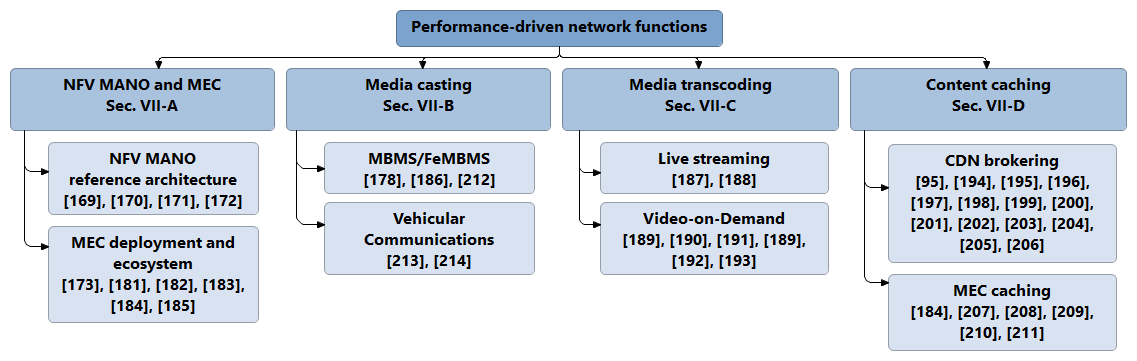
\includegraphics[width=1\textwidth,clip,keepaspectratio]{functions.png}
	\caption{Performance-driven Network Functions.}
	\label{fig:IEEECOMSTnetfunctions}
	\vspace{-0.5cm}
\end{figure}

This section presents an overview of VNF-based solutions designed to improve the performance of media streaming. These solutions employ knowledge that comes from network studies and data acquired from live monitoring of network traffic. Figure \ref{fig:IEEECOMSTnetfunctions} illustrates the major avenues that performance-driven VNF solutions take. First we introduce NFV Management and Orchestration and Multi-access Edge Computing, as VNFs rely on these paradigms introduced by European Telecommunications Standards Institute (ETSI) and embraced by 5G networks. Then, we discuss the state-of-the-art of most relevant media-related functions such as media casting, media transcoding and content caching.

\subsubsection{NFV Management and Orchestration and Multi-access Edge Computing}

Apart from the performance leaps on Key Performance Indicators (KPI) in terms of speed, capacity, mobility, and reliability, brought by 5G radio technologies, the network core is also fully engaged in a revolution, involving its own digital transformation. The concept that one network fits all is over. It is time to adapt the network according to applicable resources efficiency and delivery performance trade-offs. The goal is to allow network management systems to coordinate the systems comprising an agile, programmable and efficient network. This vision is being fueled by the transformation of network functions into dynamically controllable and configurable software components, which are virtualized exploiting cloud technologies and their scalable mechanisms, where orchestration of distributed network functions is done on top of the dynamic configuration of software systems. Going beyond, catalyzed by the network slices concept, the network would also connect groups of virtualized functions devoted to specific data flows or groups of users of specific services, handling independently Service Level Agreements (SLAs) of multiple points of presence (PoPs) over a common bare-metal infrastructure.

To achieve it, 5G network embraces NFV and VNF \cite{Liang2015} concepts and comes with a NFV Management and Orchestration (MANO) architecture \cite{ETSI2014}, standardized by ETSI.

NFV brings the primary virtualization step, providing computing, memory, storage and network resources from a bare-metal infrastructure (NFV Infrastructure or NFVI). The utilization of NFV contributes to the deployment of a network providing hardware and software decoupling. Thus, commercial off-the-shelf (COTS) hardware can be used to run every network function having a software implementation (VNF). This architecture is mainly employed by cloud vendors in order to provide Infrastructure as a Service (IaaS) solutions. Thus, hosting for systems on top of hardware and connectivity setup is performed on demand.

VNFs goes a step further in virtualization deploying specific network functions on top of NFVI.
VNFs can be deployed, configured, started or stopped in a programmable manner. Thus, VNFs are intended to enable modularity, interoperability, scalability and flexibility when a media streaming service is managed, and the generated traffic is delivered.

\begin{figure}[htp]
	\centering
	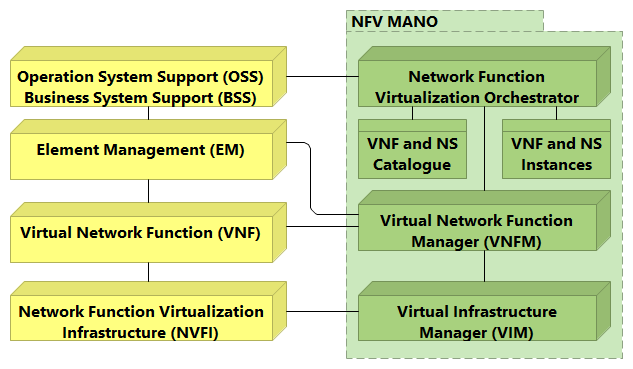
\includegraphics[width=0.5\textwidth,clip,keepaspectratio]{MANO.png}
	\caption{ETSI NFV MANO architecture.}
	\label{fig:IEEECOMSTmano}
	\vspace{-0.5cm}
\end{figure}

NFVI and VNFs are managed and orchestrated by NFV MANO, whose reference architecture is shown in Figure \ref{fig:IEEECOMSTmano}. Its functional blocks are:

\begin{itemize}
	\item Virtual Infrastructure Manager (VIM): It manages and controls physical and virtual resources (compute, storage and networking resources). Once a VNF is instantiated (VNF Instance or VNFI), it provides the VNFI with the resources it requires.
	\item VNF Manager (VNFM): It is responsible for the management of the life cycle of VNFI through the resources provided by the VIM.
	\item NFV Orchestrator (NFVO): It combines more than one VNF to create end-to-end services. Several VNFs could share VIM resources and be meant to be used for the deployment of a unique Network Service (NS), e.g., one VNF deploys the back-end and another one the front-end, the combination of the two VNFs constitute the NS.
\end{itemize}

Since 5G architecture allows for both public and private network deployment, existing NFV MANO-compliant solutions encompass both commercial and open-source alternatives for each of the three components. Some examples are Open Source MANO (OSM) \cite{OSM}, whose development is promoted by ETSI, and Open Network Automation Platform (ONAP) \cite{ONAP}, supported by Linux Foundation.

All the described technologies that turn network functions into virtualized software systems facilitate a high level of automation and orchestration by network management systems.
% which bring efficiency and intelligence to network workflows.
This trend is being deeply explored and investigated in the current generation of mobile networks (5G) and it will be key pillar for next ones (beyond 5G) and Multi-access Edge Computing (MEC) infrastructures \cite{etsi2019}. MEC architectures enable context-aware applications. It opens computing infrastructures co-located with the base stations to host services closed to the mobile users exploiting the capillary distribution of cloud computing infrastructures at the edge of the cellular Radio Access Network (RAN).

\begin{figure}[htp]
	\centering
	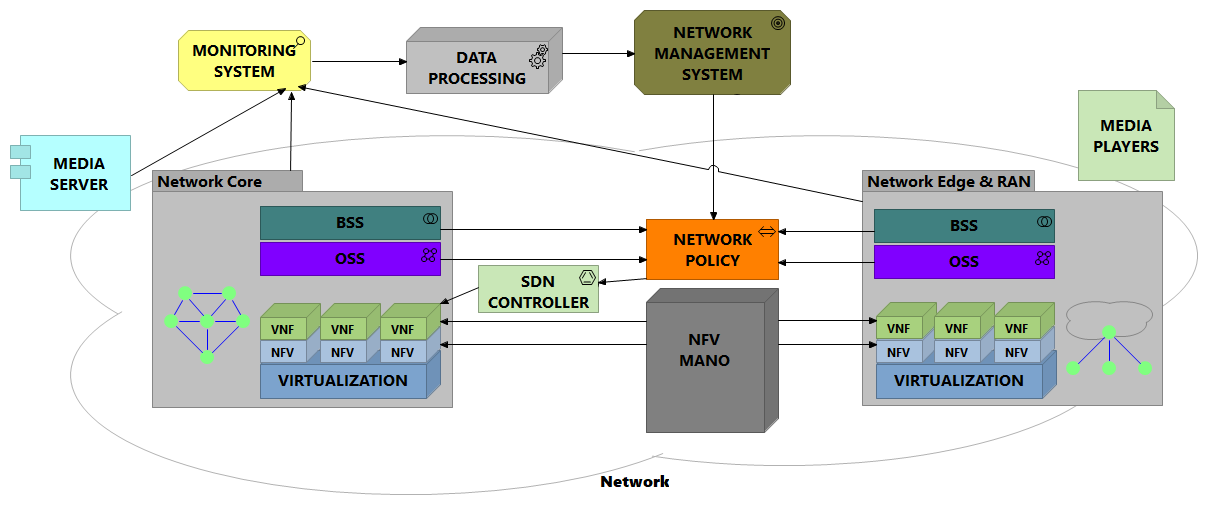
\includegraphics[width=1\textwidth,clip,keepaspectratio]{vnfmedia.png}
	\caption{ETSI NFV architecture applied to Media streaming services.}
	\label{fig:IEEECOMSTvnf4media}
	\vspace{-0.5cm}
\end{figure}

The application of NFV and VNF technologies at the edge and the evolution of the RAN towards software components boosted by open-source software, such as OpenAirInterface \cite{nikaein_openairinterface_2014} or srsLTE \cite{Gomez2016}, eases the integration of MEC services with RAN systems. These solutions implement the Mobile Packet Core (Evolved Packet Core for LTE, 5G Core for 5G) and the RAN on top of open-source hardware enabling the deployment, management and orchestration through NFV MANO of both the mobile packet core \cite{Nguyen2017, Ocampo2020} and RAN \cite{Gabilondo2020}.
A RAN deployment through NFV and VNF is usually referred as virtual RAN (vRAN). vRAN is also evolving towards the concept of Open RAN (O-RAN) \cite{openRAN}, having open interfaces and network intelligence as key enablers to manage and tailor the network based on vendors and operators' requirements. O-RAN enables multi-vendor vRAN deployments, resulting in a more competitive and richer ecosystem \cite{gavrilovska2020cloud}.
In this context, MEC is a NFV MANO-compliant platform that comes also with a specific API to access Radio Network Information (RNI) \cite{etsigsmec012}.

Figure \ref{fig:IEEECOMSTvnf4media} shows how the virtualized (NFV) and softwarized (VNF) systems at the network core and edge are monitored and orchestrated according to business and technical policies which ask for changes in the NFV MANO system or SDN controller. Thus, any dynamic changes of the network can be applied over a widely-employed technology stack. 

While focusing on the edge architecture, Figure \ref{fig:IEEECOMSTmec2} illustrates the MEC components and their interactions with the rest of the building blocks of RAN and Core Network (CN). The MEC host manages the User-plane, while the Data-plane communication is managed by the CN (LTE Evolved Packet Core or 5G Core).
Depending on whether the deployment is within an LTE or 5G network, MEC host is equipped with User-plane Serving and Packet Gateways (SGW-U and PGW-U) or User Plane Function (UPF), respectively. These components are connected directly to the base station (eNB for LTE or gNB for 5G) and provide access to Internet. Inside the MEC Host, the RNI service (RNIS) oversees collecting RAN information which is later consumed by the application VNFs. Specifically VNFs can be designed to exploit such information to increase the overall system performance.

\begin{figure}[htp]
	\centering
	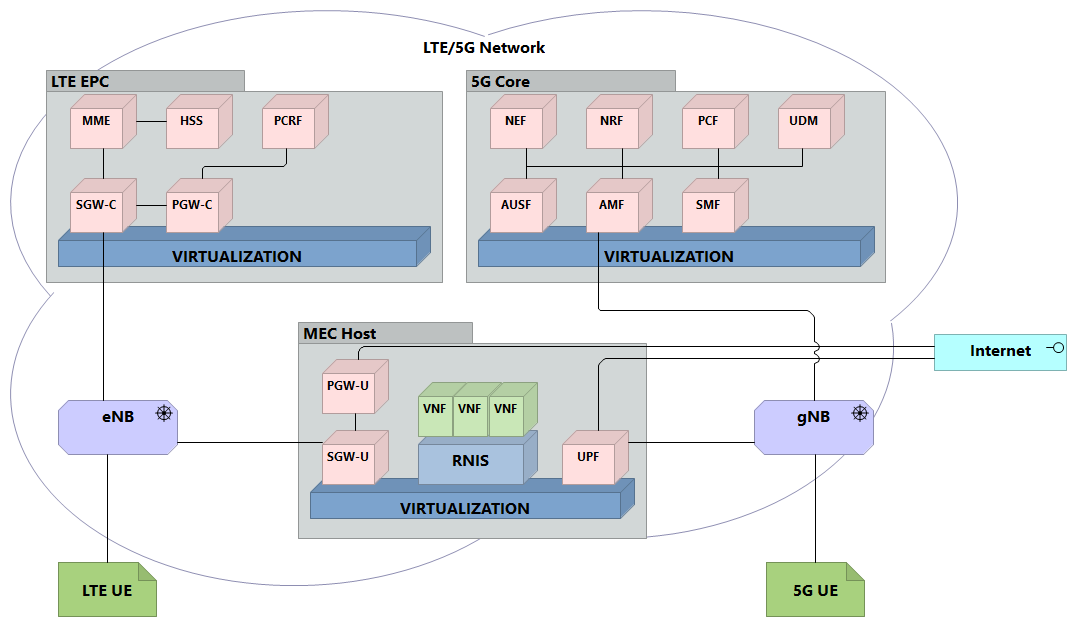
\includegraphics[width=0.8\textwidth,clip,keepaspectratio]{MEC2.png}
	\caption{MEC architecture and connection with RAN and CN.}
	\label{fig:IEEECOMSTmec2}
	\vspace{-0.5cm}
\end{figure}

Beyond this design, VNF is also applicable for media-specific network functions beyond the 5G core and RAN, involving:
\begin{itemize}
	\item media casting, in order to perform massive delivery of live data flows,
	\item media transcoding, such as streaming rate matches network available bandwidth, resulting in higher quality at destination and
	\item content caching, including storing popular data to help improved high traffic conditions, and managing alternative endpoints to balance the data requests.
\end{itemize}

All these network functions perform specialized functions of the media applications in order to improve network efficiency, saving bandwidth overheads and favoring the allocation of idle resources to other network flows, and to enhance quality of experience with enforced KPIs according to SLAs.

ETSI includes several use cases related to media streaming to be considered for MEC deployment \cite{etsigsmec002} empowering traditional media streaming applications, which are based on interaction between remote server (origin server or CDN) and client, as shown in Figure \ref{fig:IEEECOMSTmec}. MEC platform can host diverse VNFs, which exploit RNI to get a wider view of the local conditions to enhance media streaming service. In this line, some solutions, such as \cite{giannone2020, Martin2019, Li2016-2}, exploit standard RAN interfaces and data reports to conclude better decisions for media applications.

\begin{figure}[htp]
	\centering
	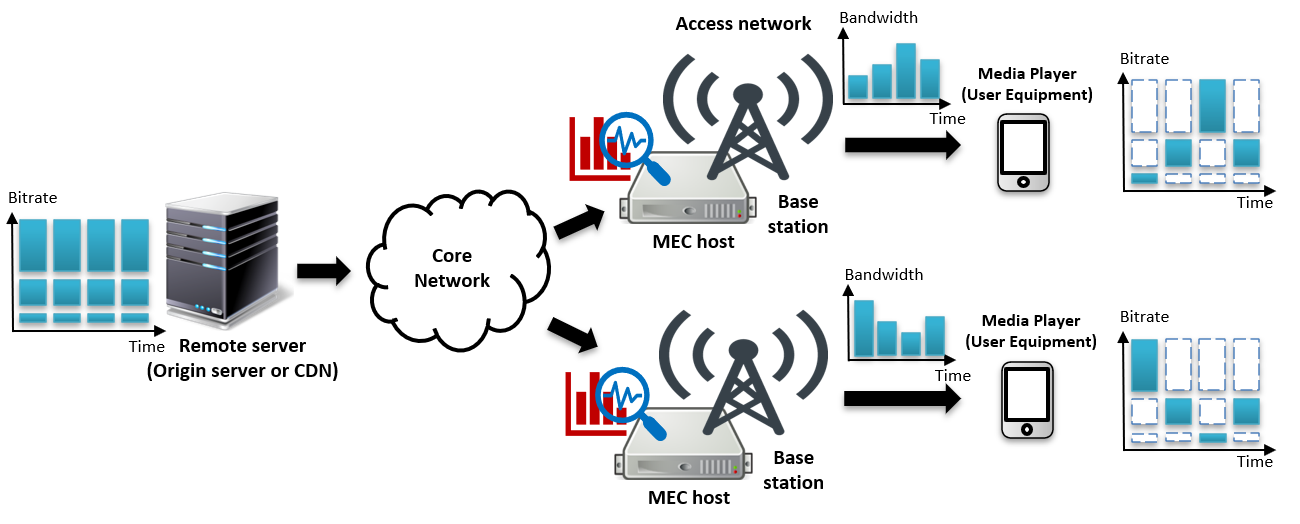
\includegraphics[width=0.8\textwidth,clip,keepaspectratio]{MEC.PNG}
	\caption{MEC-powered media streaming.}
	\label{fig:IEEECOMSTmec}
	\vspace{-0.5cm}
\end{figure}

The following sections analyze how the described core technologies of 5G %, which hold the network revolution, 
are applied to expand the network functions with core components for improved delivery of media streams, resulting with benefits in terms of enhanced quality and efficient resources utilization. Accordingly, Table \ref{tab:IEEECOMSTmedianf} compiles and classifies all the research activities exploiting 5G to support performance-aware networking. The classification highlights the main features implemented, as well as secondary aspects, as sometimes the same approach is applicable to more than one solution.
Some proposals are limited to architecture design and do not achieve a real implementation and experimentation. The implemented ones differ in terms of activation and processing approach, as they could operate in reactive or proactive manner and, in same cases, embed a processing algorithm (classic or ANN-based).
All proposed solutions aim to have direct impact on the performance of the media streaming systems, ranging from QoS and QoE enhancement to more effective business costs and energy saving. However, most of them do not provide specific validation tests, especially in terms of HAS-centric QoE metrics, or insights on applicable cost models which include business aspects or evidence on energy footprint.

\begin{table}[htp]
	\caption{Performance driven networking for media streams using 5G technologies.}
	\centering
	\label{tab:IEEECOMSTmedianf}
	\def\arraystretch{1.2}%  1 is the default, change whatever you need
	\setlength\tabcolsep{2.0pt} % default value: 6pt
	{\scriptsize
		\begin{tabular}{>{\centering\arraybackslash}m{\dimexpr0.11\textwidth-2\tabcolsep-\arrayrulewidth\relax}
			>{\centering\arraybackslash}m{\dimexpr0.11\textwidth-2\tabcolsep-\arrayrulewidth\relax}
			>{\centering\arraybackslash}m{\dimexpr0.1\textwidth-2\tabcolsep-\arrayrulewidth\relax}
			>{\centering\arraybackslash}m{\dimexpr0.1\textwidth-2\tabcolsep-\arrayrulewidth\relax}
			>{\centering\arraybackslash}m{\dimexpr0.2\textwidth-2\tabcolsep-\arrayrulewidth\relax}
			>{\centering\arraybackslash}m{\dimexpr0.15\textwidth-2\tabcolsep-\arrayrulewidth\relax}
			>{\centering\arraybackslash}m{\dimexpr0.25\textwidth-2\tabcolsep-\arrayrulewidth\relax}
		}
		\toprule
		\textbf{Main Feature} & \textbf{Secondary Feature} & \textbf{Activation} & \textbf{Processing approach} & \textbf{References} & \textbf{Network features} & \textbf{Description} \\
		\midrule
		\midrule
		Casting & - & Not Applicable & Not Applicable & \cite{Gimenez2019} & FeMBMS & Design of 3GPP architecture for media multicast \\
		Casting & - & Reactive & Not Applicable & \cite{Gabilondo2020} & FeMBMS, VNF, SDR & Virtualization of FeMBMS with SDR setup \\
		Transcoding & - & Not Applicable & Not Applicable & \cite{Doumanoglou2018} & NFV, VNF, 5G Core & Design of centralized virtual transcoder solution at 5G Core \\
		Transcoding & - & Reactive & ANN & \cite{Dutta2016} & VNF, MEC & On-the-fly transcoder at the network edge \\
		Transcoding & Caching & Proactive & Classic & \cite{Rezvani2019} & L1 MC-NOMA, MEC & Solution empowered by mulitcarrier non-orthogonal multiple access \\
		Transcoding & Caching & Reactive & Classic & \cite{Liu2021} & MEC, VNF & Transcoding and cache location in virtualized edge infrastructures \\
		Transcoding & Caching & Reactive / Proactive & Classic & \cite{Tran2019} & MEC, VNF & Transcoding and cache location when content popularity is known (proactive) or not (reactive) \\
		Transcoding & Caching & Proactive & Classic & \cite{Wang2021, Jia2019} & MEC, VNF & Transcoding and cache location based on known content popularity \\
		CDN Brokering & - & Reactive & Not Applicable & \cite{adhikari2012, adhikari2012-2, adhikari2015} & L7 & Proprietary solution for selection of CDN vendor at startup \\
		CDN Brokering & - & Reactive & Classic & \cite{otto2012, torres2011, goel2015} & L3 DNS & Performance-driven solution based on DNS resolution \\
		CDN Brokering & - & Not Applicable & Not Applicable & \cite{botteger2018, OpenCaching, frank2013, wichtlhuber2015} & L3 DNS & Design of CDN-ISP collaborative solutions \\
		CDN Brokering & - & Proactive & ANN & \cite{Viola2020} & L7, L3 & Solution for proactive CDN selection employing ANN algorithm to forecast network metrics \\
		CDN Brokering & - & Reactive & Not Applicable & \cite{EurovisionFLOW, citrix2, lightflow} & L7 & Cloud solution for cost-effective CDN switching \\
		Caching & CDN Brokering & Reactive / Proactive & Classic & \cite{viola2018} & L7, L3, MEC & Statistical solution for CDN selection (reactive) and content caching (proactive) \\
		Caching & - & Not Applicable & Not Applicable & \cite{carrozzo2018} & VNF, Orchestration & Design of virtual CDNs for media distribution \\
		Caching & - & Proactive & Classic & \cite{Tan2018} & MEC, SDR & Solution at edge exploiting radio network information \\
		Caching & Fair QoE & Reactive & Classic & \cite{Martin2019} & MEC, SDR & Solution at edge exploiting radio network information \\
		Caching & Fair QoE & Reactive & Classic & \cite{Ge2016} & MEC, SDR & Solution at edge exploiting radio network information and content popularity \\
		Caching & - & Proactive & ANN & \cite{chen2020} & MEC & Solution for proactive caching employing ANN technologies to predict popularity \\
		\bottomrule
		\bottomrule
	\end{tabular}
	}
\end{table}


\subsubsection{Media casting}

For massive delivery of common data at once, synchronously, broadcast is still much more efficient that unicast communications widely employed by cellular networks. That is why 3GPP introduced Multimedia Broadcast/Multicast Service (MBMS) specification in
Long-Term Evolution (LTE) release 9, which has been evolved towards further enhanced MBMS (FeMBMS) in release 14 to enable higher per cell bandwidth for MBMS services and simultaneous reception of both unicast and multicast services \cite{Gimenez2019}.
Furthermore, release 16 includes feedback for increased reliability \cite{3GPP2020}.

In fact, as this technology is tied to the RAN system, it has sense in some use cases as firmware/software updates, clock synchronization, alarms and massive media contents to be turned in the network edge from unicast communications to broadcast signals. This would need the support from MEC systems which will turn popular streams into broadcast flows to expand the capacity of a cell. This is feasible as manifests of HAS technologies, such as HLS or DASH, even for encrypted contents keep the manifests unencrypted allowing a simple processing to parsed them by intermediaries, such as CDNs or MEC systems, for efficient and smart media delivery.

This architecture brings three major benefits by means of attracting all the ongoing live sessions to consume the broadcast dataflow, instead of establishing concurrent unicast sessions:

\begin{enumerate}
	\item Efficiency at the radio link, as the broadcast stream reduces radio link usage. Data traffic is independent of volume of users since everyone is consuming the same broadcast signal.
	\item Optimal fidelity, as the network is able to deliver to all the audience the maximum resolution (bitrate representation).
	\item Enhanced QoE, as the media players sharing the radio-link do not have to struggle with independent adaptive mechanisms executed in each player competing for the available bandwidth. This means no bitrate or resolution changes to track time-varying network conditions and no freezes to refill the buffer.
\end{enumerate}

This approach is possible thanks to the application of virtualization and softwarization paradigms to RAN technologies, making vRAN and the containerization of some RAN network functions such as FeMBMS feasible \cite{Gabilondo2020}.

Specifically, broadcast communications are gaining relevance in the vehicular communications field as they allow synchronous provisioning of common awareness to vehicles, pedestrians and Road-Side Units (RSU) in a surrounding area. Common awareness can be essential for Cooperative, Connected and Automated Mobility (CCAM) applications related to safety of autonomous driving \cite{Ma2020}. In these applications media flows are important as the vehicles gets fitted with more camera-like sensors capturing the environment and exchanging the raw/compressed data or processed insights/summaries from on-board computer vision systems \cite{Velez2020}.

\subsubsection{Media transcoding}

Media services have become a fundamental service in 5G networks. There, as summarized in Table \ref{tab:IEEECOMSTalternatives}, HAS technologies, such as DASH or HLS, are widely employed and need the provision of several representations meaning different resolutions and bitrates \cite{Liu2021}. Thus, VNF-based transcoders are being developed under international funding initiatives aiming to empower different use cases, e.g., live 3D media streaming \cite{Doumanoglou2018} or automotive \cite{vnfTranscoders}. Here, the generation of representations at edge servers is gaining relevance to get higher efficiency by distributing the higher fidelity through the core and generating variants at the edge. This would reduce overheads in the core to send all the possible media variants. To this end, the media transcoding at the edge is essential \cite{Tran2019}, stressing the fronthaul capacity and requiring Cloud-RANs (C-RANs) or MEC systems in order to minimize the network delivery cost. Furthermore, the capillarity of the MEC systems brings a better adaptation to the local needs when transcoding to produce variants.

However, transcoding is a heavy process which needs a smart mechanism to gain efficiency. Transcoding at resource-constrained MEC server means a challenge for delay-sensitive services. Here, different works deal with the optimal position of transcoding systems in different edge hosts to respond to a distributed demand more efficiently and quickly, where players use a specific base station as a gateway linked to host and an edge server. To overcome this challenge, a mechanism for optimal request forwarding which respects the resources limitations and minimize serving latency is required \cite{Rezvani2019}. In \cite{Wang2021}, different short/long-term decisions are concluded to deal with the time-varying conditions in terms of demand and network dynamics.

Beyond the planning of such transcoding process, other approaches consider different algorithms for reactive or proactive planning \cite{Tran2019}. In this case, the dynamics have a big impact on the reaction time and forecast range. These aspects are minimized using a segment duration in the HAS stream with favor steady short-term conditions as changes comes in a segment duration-basis.

These works focus on enhancing QoS metrics while managing capacity of each processing asset. However, they do not consider heterogeneous SLAs and cost penalties to apply trade-off policies. As the GPU assets are required for \hbox{HW-accelerated} transcoding to ensure parallelization of transcoding threads and they have a big impact on infrastructure costs, this aspect should be a primary feature to evaluate.

It is important to underline that these solutions are often linked to caching strategies as both can be executed at the edge to better match the local conditions, patterns and demand features. Therefore, they design a joint strategy for transcoding processing and caching \cite{Liu2021, Tran2019, Rezvani2019, Wang2021, Jia2019}. In \cite{Dutta2016}, the authors only transcode the content on-the-fly if the content is not cached.

\subsubsection{Content caching}

%\subsubsubsection{CDN brokering}
\textbf{CDN brokering:}
Caching is the most employed network function to improve the performance when accessing online contents and, in particular, media streaming ones. In this context, a CDN is the most popular network solution aiming to provide caching capabilities. It consists of a geographically distributed network of proxy servers and data centers to provide high availability of the contents. Caching mechanisms are key inside a CDN, as CDN proxy servers work by selectively storing the content such that the users can quickly access it from nearby locations. The employment of CDN service by the CPs increased in the last years, as the number of CDN vendors increased. Furthermore, major CPs also moved to multi-CDN strategies to provide a more reliable service while streaming their contents. Thus, an improved service also generates more satisfaction among the customers. Nevertheless, how the different CDNs are employed can differ from a CP to another. Static selection of the CDN when a streaming session starts is the easiest and widely employed solution among the CPs. In 2012, this strategy was used by Netflix \cite{adhikari2012} and Hulu \cite{adhikari2012-2}, with big similarities \cite{adhikari2015}. In both cases, they were using three different CDN vendors. They used to map the player device to a CDN depending on to its location or the subscriber when the streaming session starts. Moreover, the CDN is never changed during the streaming session, even when the performances decrease.
Other solutions include client-side CDN selection \cite{otto2012} or Domain Name System (DNS)-based solutions \cite{torres2011}. Client has a privileged position to measure end-to-end QoS metrics (network bandwidth and latency) when choosing the CDN, but it has the advantage to produce an uncoordinated decision as each client selects the CDN independently from the others.
A DNS-based solution means resolving a fixed hostname owned by the CP into different IP addresses referring to several CDNs. Depending on the DNS resolution, the client receives the content from the appropriate CDN. In any case, a sub-optimal CDN server selection could lead to performance decreasing \cite{goel2015}, affecting the user's satisfaction.

In the last years, other network caching solutions are also raising to empower the delivery. The same Netflix changed its streaming strategies. It developed and deployed an in-house CDN, called Open Connect \cite{botteger2018}, to reduce the dependency from CDN vendors and streaming costs. Moreover, Open Connect is meant to be run also inside the ISP infrastructure, i.e., closer to the user, to guarantee better performances in terms of network bandwidth and latency \cite{Doan2020}. The use of Open Connect also helps Netflix and other CPs having in-house solutions to better control the resources enabled for the streaming session and to reduce the costs. Anyway, it requires a large investment to have such a solution and it could not be affordable by small CPs.

The Streaming Video Alliance (SVA) is a joint initiative which works on different aspects of media streaming and aim to standardize the employed protocols and technologies. Its membership includes some of the major world-wide agents in content production and streaming. Among its activities, the SVA Open Caching Working Group \cite{OpenCaching} oversees identifying the critical components of a non-proprietary caching system and establishing the basic guidelines for its implementation inside the ISP infrastructure. Thus, it wants to promote an architecture similar to Netflix' Open Connect, but with the advantage to be standardized.

Other collaborations between CDN and ISP are proposed in literature. In \cite{frank2013}, ISP provides the CDN provider with information concerning geographical user distribution and allows the CDN provider the possibility to allocate server resources inside the ISP network. The authors of \cite{wichtlhuber2015} use a redirection center instance inside the ISP network which intercepts the client requests and selects the appropriate CDN server. The process is transparent to the client as the redirection center employs a CDN surrogate to store the content and instructs an OpenFlow controller to migrate the traffic to the CDN surrogate.
Beyond the employment of multi-CDN solutions, there are still possibilities of improvements. CDN Brokering \cite{biliris2002} is proposed to make more effective CDN utilization in a multi-CDN environment. It redirects clients dynamically between two or more CDNs.

CDN brokers work as switching services that dynamically and seamlessly select the optimal CDN to use at any time. To achieve this, CDN brokers collect and analyze in real time the performance of the available CDNs to select the best one. Thus, network analytics have a prominent role in CDN selection, in contrast with traditional multi-CDN strategies where the same CDN is kept during the streaming session.
The approach from \cite{Viola2020} applies ANN technologies to forecast dynamic demand and changeable performance to make decisions including cost-performance trade-offs.
In this context, a representative example is Eurovision Flow \cite{EurovisionFLOW}, proposed by the European Broadcasting Union (EBU). Similar solutions are also provided by Citrix \cite{citrix2} and Haivision \cite{lightflow}.

%\subsubsubsection{Edge caching}
\textbf{Edge caching:}
In \cite{viola2018}, a MEC proxy retrieves media streaming metrics of video players at the access point and CDNs performance metrics to enhance DASH media streaming. The MEC proxy evaluates the performance of different CDNs and switches players' sessions when a CDN is under-performing and cannot support the demanded traffic. Moreover, it features a local edge caching to reduce network traffic. Recurrent content is downloaded and cached once for every player. In \cite{carrozzo2018}, a similar MEC cache is proposed for empowering the delivery.

With a deeper integration with RAN interfaces, in \cite{Tan2018} and \cite{Martin2019} the MEC cache is improved by exploiting RNI. The media segments and representations are selectively cached depending on the network state. In \cite{Ge2016}, both RNI and knowledge of segment popularity are employed to decide the segments to cache.
Moving from a reactive to a proactive approach, the authors of \cite{chen2020} empower the edge cache with neural collaborative filtering to predict content popularity. The predictions are exploited to proactively cache the content at the MEC, as more content popularity means higher probability to be requested by the users.

\subsection{Challenges of Virtual Network Functions for Media Streaming}
\label{sec:IEEECOMSTchallenges}

VNF solutions play a significant role in the successful deployment of 5G networks. This is backed by evidence, especially for supporting rich media applications such as multimedia streaming, as described in section \ref{sec:IEEECOMSTfunctions}. However, VNF applications still require some challenges and open issues to be addressed, as shown in Figure \ref{fig:IEEECOMSTchallenges}. This section discusses and classifies these challenges around some key features studied in relation to 5G networks and presents the open issues in the context of the 6G networks' roadmap.

\begin{figure}[htp]
	\centering
	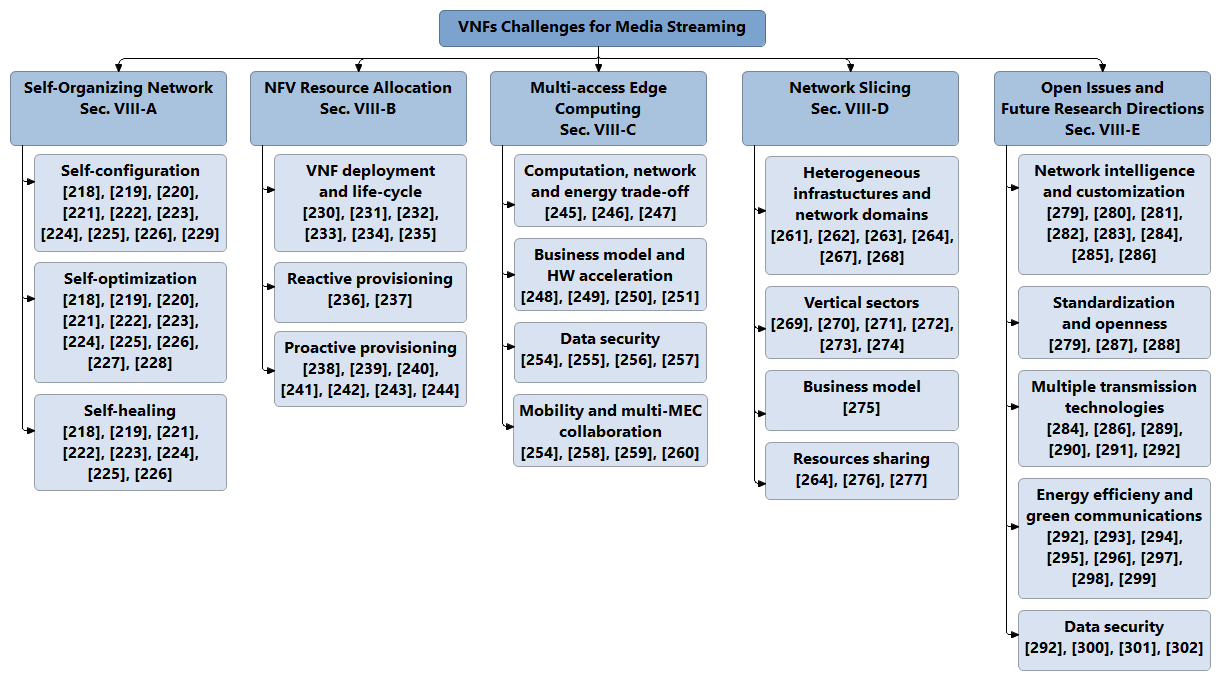
\includegraphics[width=1\textwidth,clip,keepaspectratio]{challenges.png}
	\caption{Virtual Network Functions Challenges for Media Streaming.}
	\label{fig:IEEECOMSTchallenges}
	\vspace{-0.5cm}
\end{figure}

\subsubsection{Self-Organizing Networks}

Agile deployment and life-cycle management of VNFs exploiting a NFV MANO architecture are essential features to satisfy the expectations of smart 5G networks, but further research is still ongoing to increase network automation. In this context, the Self-Organizing Network (SON) paradigm \cite{ETSI2020} represents a next step to achieve a fully virtualized and automated network, as it empowers the network with specialized decision-making algorithms which monitor network resources and traffic patterns, and autonomously take actions to enforce or optimize network operations \cite{Aliu2012}. SON capabilities were initially meant to be included as add on features of LTE, as 3GPP Release 8 started defining LTE and already set the basis for SON concepts and requirements \cite{Hu2010}.
However, SON is expected to enhance 5G network management providing automation to cope with increasing network complexity \cite{Moysen2018}.

Specifically, in the media streaming context, SON should provide the required network resources and guarantee target QoS or QoE scores when delivering media streams. More generally, SON turns static networks into dynamic ones by configuring network parameters, optimizing the allocated resources and fixing or preventing issues in real time.

\begin{table}[htp]
	\caption{SON categories and use cases.}
	\centering
	\label{tab:IEEECOMSTusecases}
	\def\arraystretch{1.2}%  1 is the default, change whatever you need
	\setlength\tabcolsep{2.0pt} % default value: 6pt
	{\scriptsize
		\begin{tabular}{>{\centering\arraybackslash}m{\dimexpr0.25\textwidth-2\tabcolsep-\arrayrulewidth\relax}
				>{\centering\arraybackslash}m{\dimexpr0.25\textwidth-2\tabcolsep-\arrayrulewidth\relax}
				>{\centering\arraybackslash}m{\dimexpr0.25\textwidth-2\tabcolsep-\arrayrulewidth\relax}
			}
			\toprule
			\textbf{Self-configuration} & \textbf{Self-optimization} & \textbf{Self-healing} \\
			\midrule
			\midrule
			\begin{itemize}[leftmargin=*]
				\raggedright
				\itemsep0em
				\item IP address \& connectivity
				\item neighbour \& context discovery
				\item radio access parameters
				\item policy management
			\end{itemize}
			&
			\begin{itemize}[leftmargin=*]
				\raggedright
				\itemsep0em
				\item load balancing
				\item resource selection
				\item caching infrastructure
				\item coverage \& capacity
				\item radio interference management
				\item mobility \& handover
			\end{itemize}
			&
			\begin{itemize}[leftmargin=*]
				\raggedright
				\itemsep0em
				\item fault detection
				\item fault classification
				\item countermeasures operations
			\end{itemize}
			\\
			\bottomrule
			\bottomrule
		\end{tabular}
	}
\end{table}

A SON-enabled system can accomplish tasks belonging to three categories: self-configuration, self-optimization and self-healing \cite{Aliu2012}.
Self-configuration techniques adjust network operational parameters to change network behavior and rules, according to specific business policies and node neighborhood context.
Self-optimization strategies are dynamically applied to ensure that the network performance is near optimal. They include real-time network monitoring and performance metrics processing to proactively apply enhancement operational parameters. Self-optimization techniques can be applied in many areas: load balancing, resource selection, caching infrastructure, coverage and capacity, radio interference management, mobility and handover.
Last, self-healing is necessary to generate a prompt reaction when faults, failures or any operational range violations in the network occur. The objective is to continuously monitor the system and ensure a fast and seamless recovery, whatever reason causes the failure. In case of a failure event, self-healing functions detect (fault detection) and diagnose (fault classification) it. Then, according to applicable policies and current setup, the appropriate countermeasure are applied to reestablish the desired network performance.

All these SON flavours need actionable data to process decision making algorithms. It is therefore very important to collect and exploit network data. Current networks are ready to probe and provide a huge amount of data. However, it is clear that specialized intelligence needs to be deployed within the network to infer valuable and useful information from the collected data \cite{Imran2014}. Such information helps taking automatic actions to reach, recover or even improve the network performance. In the context of media streaming, it means that the SON paradigm has the potential to increase the QoS/QoE, while decreasing the business costs and energy consumption to maintain the network. In this context, the use of ML techniques will become prominent, even if the selection of the right algorithm is not trivial and depends on the considered use case \cite{Klaine2017, Moysen2018}. Table \ref{tab:IEEECOMSTusecases} shows the most common use cases belonging to the three SON categories, as seen from the network operator's perspective. Some SON applications are already provided by network vendors included in their commercial hardware equipment. Some examples are HCL's SON \cite{HCLSON}, Nokia's EdenNet \cite{NokiaSON} and Ericsson's SON Optimization Manager \cite{EricssonSON}.

In any case, SON systems need to have a wider view of the delivered traffic beyond the metrics from the network functions and including service domain. It means that operated SON policies are usually steered by network statistics rather than application characteristics. Nevertheless, the  communication dynamics of applications delivered on top of the network have an impact on network performance. Thus, the authors of \cite{Ouyang2020} propose to design an application-driven SON in order to widen the view with both network performance and user's QoE metrics. When considering media streaming applications, data are available from network functions in the path and from playback devices. Thus, data exploitation inside a SON-enabled system needs further investigation, as the multi-domain data exploitation is still underexplored. Few solutions are available in the literature that apply a SON paradigm to media streaming scenarios. The authors of \cite{Khan2001} propose a SON-enabled media transcoder to be deployed within the network. In \cite{Singhal2021} the authors introduce a self-organizing Unmanned Aerial Vehicle (UAV)-based communication framework for media streaming.


\subsubsection{NFV Resource Allocation}

The deployment of a VNF over a distributed platform requires the allocation of network and computing assets to be provisioned to host the VNF. Network and computing resource allocation is a challenging feature whose interest is raising and focusing on VNFs deployment and life-cycle management \cite{Herrera2016}.
In this context, the NVFO is in charge of selecting the appropriate resources, among the available ones at the NVFI, when deploying a VNF,
% and managing its life-cycle.
which is usually referred to as the NFV resource allocation (NFV-RA) problem. The NFV-RA includes three stages \cite{Herrera2016}: VNF Chain Composition (VNF-CC), VNF Forwarding Graph embedding (VNF-FGE) and VNF Scheduling (VNF-SCH).

VNF-CC deals with the composition of several VNFs to be deployed jointly by the NFVO. How the traffic flows between VNFs is also described trough the definition of VNF Forwarding Graphs (VNF-FG). Thus, any network service %NS is meant to be 
can be considered as composed of a set of VNFs and VNF-FGs. Each VNF executes a small function of the entire application or service \cite{Xie2016}.
VNF-FGE focuses on how to embed the VNFs and VNF-FGs into the infrastructure. It aims to find suitable resources and locations where to allocate the VNFs in NFVI. At this stage, resource selection and optimization must be accomplished with regard to the specific constraints defined by SLA \cite{Schardong2020}.
Finally, VNF-SCH determines how to schedule the processing operations of the deployed VNFs \cite{Riera2014}.

When the VNFs are already deployed and running, the required resources vary during their life-cycle, as they depend on user demand of the running function provided by the VNFs. Allocated resources could be optimized to fit with the variable demand by the user. Increasing or decreasing the allocated resources means the VNFs also need to dynamically scale up/down. Then, an efficient orchestration and automation of the VNFs requires supporting this dynamic allocation of resources.
This assumption was already envisioned when designing the NFV MANO architecture \cite{Adamuz2018}, where mechanisms to scale are essential to enable a flexible management of the running services.

However, the easiest and fastest approach consists of employing an over-provisioning strategy, where the amount of allocated resources for each VNF is larger than what is required. In case of experiencing an increasing demand, the VNF can manage overheads without any intervention as long as the allocated resources are not exceeded. This approach is operationally effective, but inefficient in terms of OPEX and energy consumption generated by the allocated resources which are not actually employed. This means that this approach is not cost-effective, as it is clear that adjusting the resources allocated for the VNF to the actual demand would avoid over-provisioning and reduce costs.
Employment of dynamic provisioning strategies results in OPEX reductions for network operators and/or service providers \cite{Hernandez2015}.

Enabling dynamic resource allocation for VNFs allows scaling up and down and therefore coping with network traffic fluctuations and changeable demands from connected users. Dynamism, scalability and automation are important features for resource management \cite{Mijumbi2016}.
Changes in resource allocation should be applied according to real-time network traffic and service demands.
Dynamic resource allocation can be performed in reactive or proactive manners. Simple solutions involve a reactive provisioning approach which means changing the allocated resources to react when traffic and/or demand change.
In \cite{Wang2016} the authors design an online algorithm for VNF scaling in cloud data centers. The authors of \cite{Ghaznavi2015} aim to minimize the OPEX by considering the trade-off between bandwidth and host resource consumption under diverse workload variations.
All these reactive solutions have the advantage of a simple design, as there is no need for any complex algorithms for provisioning. On the other side, such an approach does not prevent any network issues or service faults from happening, affecting the services. %This is as the algorithms react to the issues and not foresee them and try to prevent them.

A more sophisticated approach consists of proactive provisioning where the future traffic and/or demand is predicted. Being able to foresee the amount of resources to be allocated constitutes a great benefit, as it enables to avoid network issues or service faults by proactively resizing the employed resources and scaling the deployed VNFs. In such a context, the problem of service demand prediction constitutes a mayor challenge. Most of the literature on demand prediction employs ANN algorithms \cite{Tedjopurnomo2020, Sandhir2008}. However, the application of such algorithms in practical solutions is limited, being mostly theoretical. %in the actuation stage.

Among the most innovative solutions proposed, \cite{Fei2018} describes a novel FTRL online algorithm for VNF provisioning which handles workload fluctuations. The solution in \cite{Mijumbi2016-2} employs an ANN algorithm to predict future resource requirements for each VNF contributing to a network service. The authors of \cite{Zhang2017} propose the POLAR algorithm, which combines online learning and online optimization of proactive provision resources with VNFs provisioning, while the VNFs chaining in a network service is ignored. In \cite{Huang2019} a proactive failure recovery is proposed when considering VNF deployed at distributed edge computing nodes. In \cite{Dieye2018} a proactive VNF chaining aims to find the optimal number of VNFs and their location inside a CDN in order to minimize costs. Finally, the authors of \cite{Moreno2019} propose a multi-layer resource allocation solution, which aims to proactively provide resources to the VNFs deployed in several VIMs and network resources between VIMs.

\subsubsection{Multi-access Edge Computing (MEC)}

MEC represents a novel technological solution integrated in 5G networks to bring computation closer to the user. %However, a wide-accepted commercial deployment is not available yet. 
MEC infrastructures create new potential revenue flows to network operators opening their edge infrastructures to host specialized services at network edge. 
%This approach gains the local view of the radio link status not visible for the central media server, the capillarity meaning less resources to serve just local sessions and lower latency thanks to the proximity to the users. 
There are many aspects which require investigation to achieve a complete integration of MEC into the current network architecture and services. However some avenues are already seen as highly beneficial for MEC deployment and use.
For instance, media streaming is a key application of MEC solutions, as ETSI considers it as one of MEC core use cases \cite{etsigsmec002}. 
MEC platforms can host edge services to empower media streaming applications, which traditionally were based on server-client communications. As explained in the previous section, MEC and VNFs enable the deployment of innovative media-related services such as media casting, media transcoding and content caching.

More specifically, MEC resources are exploited by both the server and clients to offload computation tasks \cite{Ndikumana2017, Beck2015}.
Offloading server tasks targets reducing network traffic and latency, as the processing is performed close to UEs. MEC resources are shared between different service providers, but how the resources are distributed among different service providers is still undefined. The authors of \cite{Ndikumana2017} propose to allocate MEC resources proportionally to the demanded resources and payment of each service provider.
If an UE offloads tasks to the MEC host, it reduces not only the device computation load, but also its power consumption, as computing-intensive tasks heavily impact on the battery duration. In \cite{Beck2015}, a video telephony application employs MEC to encode the content. It reduces processing operations at the UE, but increases network traffic since uncompressed raw content is sent to the base station. The authors focus on power consumption, but they do not consider operational costs generated by using the MEC platform.
In general, how to balance network traffic, power consumption and operational costs trade-off needs to be studied. In \cite{Sun2020}, optimization of the allocation of both computing and network resources is discussed, while taking into account the energy efficiency. Even in this case, operational costs are not considered in the optimization problem. In general, business aspects
% are complicated to discuss
raise complex discussions
due to the lack of a clear business model \cite{Ahmed2017}. MEC needs a business model equivalent to the one applicable in cloud computing infrastructures. However, unlike cloud computing, the decentralized location and utilization of shared resources between services makes the cost model more complex. Resource accounting and monitoring have to also be determined in order to create a complete business model. The debate on the business model is even more intricate if we consider hardware-acceleration assets, such as GPUs, required to accomplish critical tasks where general-purpose hardware (CPU) has limitations \cite{Liu2019}. Some works suggest to employ Field-Programmable Gate Array (FPGA) approaches instead of GPU solutions due to their reduced price and power consumption \cite{Biookaghazadeh2018, Colbert2021}, but this possibility is again underexplored.

% A collaborative cache allocation and computation offloading at distributed is proposed in \cite{Ndikumana2017}, where the MEC resources are allocated to different services proportionally to their demands and payment.
% In \cite{Beck2015}, video telephony is empowered with MEC. The UE offloads the video encoding to the MEC server in order to reduce its power consumption, as the encoding operation is a computing-intensive tasks which heavily impact on the battery duration. As a backwards, offloading the encoding results in increased traffic between the UE and the base station.

Regarding to accessible information at MEC, the API to communicate with RNIS \cite{etsigsmec012} has been recently standardized and its development is on going \cite{Arora2019, Tomaszewski2020}. It means that services running at the MEC host cannot be further optimized. When RNIS implementations will be available, edge services could embed more complex and precise algorithms (classic or ML models), aiming to exploit RNI in order to improve their operations and the performance of the overall system. However, improved capabilities due to RNI exploitation raise some security concerns on how to manage information at MEC hosts, an aspect that needs further investigation \cite{Jiang2021, Gur2020}. In order to exploit a MEC decentralized approach, the deployment of location-aware services is necessary. Thus, mechanisms for user privacy protection and anonymity are needed. Moreover, modification of the networks to introduce MEC capabilities opens the door for potential attacks, including DDoS attacks, malware injection, authentication and authorization attacks \cite{Roman2018, Xiao2019}.

Mobility remains another major concern and is becoming critical, as the explosion in availability and type of mobile devices (e.g., smartphone and tablets) involves an increasing number of UEs to be served.
% The UE can move and having to change the connection from a MEC host to another.
The same way the connectivity is guaranteed when moving from a cell to another in a cellular network, migration support for MEC services is also required. Consequently, the investigation on a multi-MEC cooperation should be addressed in order to guarantee seamless migration of sessions across MEC servers \cite{Jiang2021, Shahzadi2017}.

From the perspective of media services, user QoE plays an important role and a wide MEC deployment definitely should target it, especially as transcoding and caching capabilities would be provided closer to UEs. %Anyway, it may result economically unfeasible. 
How to balance the cost of MEC-based caching and transcoding and provision of high user QoE is an important direction for future research \cite{Jiang2021}.
Moreover, it becomes relevant the ability to find suitable locations where MEC instances should be deployed, as it may affect the fulfilment of the demanded requirements. It is especially true for low latency multimedia services, where the distance between the MEC host and UE affects the overall delay \cite{MartinPerez2019}.
Finally, content caching mechanisms in the network have been studied both at the core and at the edge, but a convergent solution has not identified yet. Caching solutions that integrate both core and edge caching could result in better network performance in terms of the energy
consumption, network throughput, latency, and user QoE \cite{Yao2019}.

\subsubsection{Network Slicing}

While NFV-RA is limited to provide NFVI resources deployed for a specific section of the network (CN or RAN/MEC), network slice has a wider scope, as it is able to provide network and computing resources even across different networks. Network slicing \cite{Foukas2017, Afolabi2018} is introduced in 5G networks as a solution involving several virtual/logical networks (slices) on top of a common physical network, where each virtual/logical network delivers the traffic generated by a specific service \cite{Nakao2017, Rost2017}. It can be considered that a network slice is associated with a set of network resources and VNFs, which can be provided by that slice. In this context, NFV MANO and SDN play an important role, especially in the deployment and management of network slices \cite{Ordonez2017, Zhang2019-2}. NFV MANO enables life cycle management and orchestration of the VNFs, while SDN allows for the configuration and control of the routing and forwarding planes of the underlying network infrastructure, providing communication between the deployed VNFs. This results in a logical network of resources and VNFs built over a common underlying physical infrastructure, 
% provided at RAN, backhaul/trasnport network and CN,
separated into diverse network slices. Each network slice provides the service as an end-to-end connectivity, meaning that network slicing provisioning refers to three different aspects: at the air interface, in the RAN and in the CN \cite{Kotulski2017, Li2016}.

Network slicing at the air interface refers to partitioning physical radio resources (physical layer or L1) into subsets of several physical resources, each one for a different network slice, then mapping into logical resources to be provided to the Medium Access Control (MAC) sublayer at the datalink layer (or L2) and higher layers.

In the RAN, network slicing changes RAN operations, including MEC-operated ones, such as device association and access control, from a cell-specific perspective to a slice-specific one. Thus, the RAN operations are service-oriented instead of physical cell-oriented. Configuration of control and user planes is tailored and/or tuned considering the requirements of each slice individually. Then, factors such as QoS requirements, traffic load or type of service/traffic are prominent when operating the RAN.

Finally, network slicing in the CN enables the definition of vertical networks, where each one aims to support a service belonging to a specific vertical industry. NFV MANO and SDN have a higher impact in this aspect of the network, where each vertical industry should be able to run its VNF-specific solutions. CN needs flexible management to enable resource scalability and migration when required by the network traffic associated with a service.

A videoconferencing system is deployed in \cite{Alemany2019} through the deployment of two different slices to split audio and video transmissions, as they have different requirements in terms of network throughput. 
In \cite{wang_enable_2019}, the authors focus on the eHealth vertical, where services are typically media-rich and mission-critical and are high QoS demanding. Then, a MEC-based application, empowered with end-to-end network slicing, is designed and developed to enable in-ambulance applications. The application is accessed by paramedics in the ambulance and sends audiovisual data to the hospital/doctor. The same vertical is addressed by \cite{Celdran2019} to enable a real-time communication between hospital staff and patients.
In \cite{Campolo2017} and \cite{Mei2019}, applications of network slicing for Vehicle-to-Everything (V2X) services are investigated. Different use cases are considered in a vehicle, including related to safety and traffic efficiency, autonomous or tele-operated driving, media \& entertainment and remote diagnostics. Each use case means different requirements in terms of latency, throughput and communication reliability. Consequently, different network slices with different configurations are required on top of the same physical network of resources.
The authors of \cite{Kurtz2018} present several use cases belonging to different verticals, such as protection and smart metering in the smart grid sector, %floating 
car and passenger data exchange %and passenger Internet 
in an intelligent transportation system and best-effort data delivery in a multimedia system. Each use case and vertical sector requires different capabilities in terms of latency and throughput. The different types of traffic are prioritized by splitting them into specialized network slices.

Network slicing-related research has increased importance in the current 5G network context. %Some issues to be solved and 
Ongoing challenges %are present 
include solutions to allow wide employment and operation of slices for different industry verticals. 
Most of slicing operations relate to the exploitation of resources provided by the network operator, but the effects of changes in network operator's business models for operating network slicing are unknown \cite{Barakabitze2019}.
The increase in the number of devices belonging to different verticals and their mobility management in the presence of different technologies (LTE, 5G, Wi-Fi) also need further investigation \cite{Zhang2017}.
An end-to-end network slice implies that slice segments potentially stretch across different administrative domains. There are two requirements in order to achieve a unified control of the network slice. First, an exchange point that performs the resource negotiation between different administrative domains is necessary to enable multi-domain slices. Then, standardized APIs should make transparent the underlying domains and simplify the negotiations to provide the control on the slice \cite{Afolabi2018}.
Finally, network slicing leverages algorithms to accommodate applications with widely diverse requirements over the same physical network. Thus, complex algorithms are necessary for deciding how to efficiently allocate, manage, and control the physical resources to be shared across diverse slices \cite{Vassilaras2017}. Concerning these algorithms, the application of ML in network systems is capturing increased research attention lately and this trend is expected to continue in the future \cite{Fadlullah2017}.

\subsubsection{Open Issues and Future Research Directions}

The benefits of virtualization for media streaming communications will increasingly evident in the next few years, as the 5G coverage will be extended. Complementary technologies such as MEC, SON and network slicing are still not fully integrated. Further efforts in integrating all these new paradigms and/or architectures are envisioned to provide a more efficient and intelligent network \cite{o-ran_integration}.

ML-powered network intelligence to manage NFV and VNFs is only partially achieved in 5G networks, but it will be also a key factor for the future 6G networks \cite{zhou2020service}. The concept of Intent-Based Networks (IBN) \cite{wei2020intent} means employing ML solutions to transform business intents into network configuration, operation, and maintenance strategies. In order to meet the massive service demands and overcome limitations due to time-varying network traffic, the network can continuously learn and adapt to the time-varying network environment based on the massive collected network data in real-time. An intelligent-native network exploits ML algorithms to improve its capabilities and reduce the business costs for service deployment and management \cite{monteil2020resource, chen2020edge}. The advantages of an intelligent-native network are two-fold. First, the network can analyze user’s behavior in real-time and autonomously learn its needs to predict its future behavior. Then, user's information can be employed for network customization to achieve a user-centric network \cite{wang2019intelligent}. Second, the network can met changing requirements of a network service during its life-cycle by autonomously matching the requirements to the corresponding network communication, computing and caching assets. This is also valid for new emerging services. Holographic (AR and VR) and haptic communications are meant to be wider available thanks to the future 6G network \cite{bhat20216g}. Moreover, the global COVID-19 pandemic is accelerating the digital transformation of multiple and heterogeneous verticals, such as development of new services for smart cities and innovation in the eHealth including telemedicine, medical and thermal imaging, and robotics for medicine practice \cite{allam2021future, akhtar2020shift}. 

Openness is also an important aspect to achieve flexible network and services \cite{zhou2020service}. Having open network platform and interfaces (O-RAN, NFV MANO, SDN, etc.) allows interconnection and interoperability of different vendors, which is essential for sharing a physical infrastructure. Thus, agents of diverse vertical industries may deploy their private physical infrastructure and manage it though NFV MANO solutions and SDN controllers independent from public networks operated by mobile network operators \cite{rostami2019private}. Standardization process will continue in the next years to fulfil the remaining gaps and guarantee interoperability of heterogeneous implementations of open network solutions \cite{BONATI2020107516}.

The cooperation of different physical networks will also attract attention. Multiple Radio Access Technology (multi-RAT) aims to employ different access network to improve the overall connectivity \cite{galinina20155g}. Its application to improve media streaming is already being investigated \cite{basaras2020multicast, borst2017dynamic}, but new transmission solutions based on space, UAV-based and underwater communications will be integrated with terrestrial ones \cite{bhat20216g, akhtar2020shift}. Flexibility to operate the network at any level (spectrum/band, physical and MAC, etc.), despite the different involved technologies, will be imperative \cite{yazar6g}.

Energy efficiency and green communications \cite{huang2019survey} are envisioned to enable more sustainable networking \cite{renga2018self}. Energy efficiency concerns are also relevant for media streaming services \cite{abou2013predictive, mehrabi2019energy}. Here, low-power wireless devices could harvest energy from the available high-power radio waves \cite{yazar6g}. Thus, battery-free implementations will be an interesting topic to be further explored in different use cases, e.g., IoT \cite{xu2018practical} and media streaming communications \cite{naderiparizi2018towards, saffari2019battery}.

Finally, the growth of network and media traffic will have consequences for security. Critical media use cases, e.g., eHealth applications \cite{al2019ehealth} and autonomous driving systems \cite{cui2019review}, need to be secured with security mechanisms which will complement the conventional cryptography-based ones. Increasing security will be assured with the design of cross-layer algorithms to protect the transferred information \cite{yazar6g, wang2020security}.

\subsection{International Initiatives}
\label{sec:IEEECOMSTinternational}

\begin{table}[htp]
	\caption{Major SDN/NFV related research activities.}
	\centering
	\label{tab:IEEECOMSTresearchproj}
	\def\arraystretch{1.2}%  1 is the default, change whatever you need
	\setlength\tabcolsep{2.0pt} % default value: 6pt
	{\scriptsize
		\begin{tabular}{>{\centering\arraybackslash}m{\dimexpr0.45\textwidth-2\tabcolsep-\arrayrulewidth\relax}
			>{\centering\arraybackslash}m{\dimexpr0.1\textwidth-2\tabcolsep-\arrayrulewidth\relax}
			>{\centering\arraybackslash}m{\dimexpr0.2\textwidth-2\tabcolsep-\arrayrulewidth\relax}
			>{\centering\arraybackslash}m{\dimexpr0.25\textwidth-2\tabcolsep-\arrayrulewidth\relax}
		}
		\toprule
		\textbf{Project} & \textbf{Time period} & \textbf{Area of concern} & \textbf{References} \\
		\midrule
		\midrule
		CogNet (Building an Intelligent System of Insights and Action for 5G Network Management) & 2015-2018 & Architecture& \cite{noauthor_cognet_nodate, ben_yahia_cognitive_2017, assem_machine_2016} \\
		SELFNET (Framework for Self-Organized Network Management in Virtualized and Software Defined Networks) & 2015-2018 & Architecture& \cite{noauthor_selfnet_nodate, celdran_enabling_2017} \\
		SliceNet (End-to-End Cognitive Network Slicing and Slice Management Framework in Virtualised Multi-Domain, Multi-Tenant 5G Networks) & 2017-2020 & Architecture & \cite{noauthor_slicenet_nodate, wang_enable_2019, salva-garcia_scalable_2020} \\
		SoftFIRE (Software Defined Networks and Network Function Virtualization Testbed within FIRE+) & 2016-2018 & TestBeds & \cite{noauthor_softfire_nodate, lake_virtualising_2017} \\
		FLAME (Facility for Large-scale Adaptive Media Experimentation) & 2017-2020 & TestBeds & \cite{noauthor_flame_2017, haensge_cloud-native_2019}\\
		5GTango (5G Development and validation platform for global industry-specific network services and Apps) & 2017-2020 & TestBeds & \cite{noauthor_5gtango_nodate, peuster_introducing_2019, soenen_empowering_2019} \\
		%5G-Xcast (Broadcast and Multicast Communication Enablers for the Fifth-Generation of Wireless Systems) & 2017-2019 & Application Verticals & {[}2020 SAILY{]}, {[}2020 MI{]}, {[}2017 5GXCASTWEB{]} \\
		5G-Media (Programmable edge-to-cloud virtualization fabric for the 5G Media industry) & 2017-2020 & Application Verticals & \cite{noauthor_5g-media_nodate, alvarez_edge--cloud_2019, breitgand_towards_2018} \\
		5Growth (5G-enabled Growth in Vertical Industries) & 2019-2021 & Application Verticals & \cite{noauthor_5growth_nodate, li_5growth_2021} \\
		%5G-VICTORI (VertIcal demos over Common large scale field Trials fOr Rail, energy and media Industries) & 2019-2022 & Application Verticals & \cite{noauthor_5g-victori_nodate, ziegler_improving_2020} \\
		5GCity (A Distributed Cloud and Radio Platform for 5G Neutral Hosts) & 2017-2020 & Application Verticals & \cite{noauthor_5gcity_nodate, colman-meixner_deploying_2019} \\
		OpenAirInterface Software Alliance & 2014- & Development Platforms & \cite{noauthor_openairinterface_nodate, nikaein_openairinterface_2014} \\
		Mosaic5G & 2016 - & Development Platforms & \cite{noauthor_mosaic5g_nodate, nikaein_mosaic5g_2018} \\
		O-RAN Alliance & 2018- & Development Platforms & \cite{noauthor_openairinterface_nodate, openRAN} \\
		\bottomrule
		\bottomrule
	\end{tabular}
	}
\end{table}

Employing VNFs for media streaming is a research topic that has attracted the attention of international organizations and international funding programs for many years now. Recently, the European Commission has funded numerous research projects aiming at developing and implementing VNFs for different research scenarios and vertical industries. Table \ref{tab:IEEECOMSTresearchproj} summarizes the most relevant actions. The project list includes initiatives targeting generic architectural design (i.e., CogNET \cite{noauthor_cognet_nodate}, SELFNET \cite{noauthor_selfnet_nodate} and SliceNet \cite{noauthor_selfnet_nodate}), activities building testbed environments and pilot environments for use case definition and testing (FLAME \cite{noauthor_flame_2017}, SoftFIRE \cite{noauthor_softfire_nodate} and 5GTango) \cite{noauthor_5gtango_nodate}, projects targeting specific application verticals and developing required functionalities (5G-Media \cite{noauthor_5g-media_nodate}, 5Growth \cite{noauthor_5growth_nodate}, 
5GCity \cite{noauthor_5gcity_nodate}) and finally international software communities to provide open-source platforms (OpenAirInterface Software Alliance \cite{noauthor_openairinterface_nodate}, Mosaic5G \cite{noauthor_mosaic5g_nodate} and O-RAN Alliance \cite{noauthor_o-ran_nodate}).

Regarding architectural definition, SELFNET H2020 project designed and tested an autonomous network management framework capable of the automatic detection and mitigation of common failures in the network \cite{celdran_enabling_2017}. Among others, it proposed the smart integration of state-of-the-art technologies in NFV. One of the outcomes is presented in \cite{Nightingale2016}, where the SELFNET framework preserves the health of the network maximizing the QoE and minimizing the end-to-end energy consumption. SliceNet project addressed both management and control planes of network slicing to leverage QoS for sliced services \cite{chang_slice_2018}. The project proposed an integrated network management, control and orchestration framework and applied the concept to a variety of use cases. One of those cases, related to multimedia health services is described in \cite{wang_enable_2019}, where demanding QoS requirements (i.e., latency) need to be fulfilled. The network intelligence topic is tackled by CogNET, a project that focused on realizing the well-known control loop MAPE (Monitor, Analyze, Plan and Execute) with Machine Learning techniques and policy-based mechanisms for a vision of softwarized 5G networks. COGNET validated its vision in different use cases that include SLA Enforcement and Mobile Quality Predictors \cite{assem_machine_2016}, \cite{ben_yahia_cognitive_2017}. 

A second group of projects aimed at creating platforms and testbed environments where specific use cases, applications, algorithms, and interoperability solutions could be designed and validated. FLAME stands out in this area as a facility for experimenting large scale experiments in the field of Adaptive Media. Since 2017, FLAME has hosted different proposals \cite{haensge_cloud-native_2019} to offload proactively video content to the edge of the network on an SDN/NFV environment. FLAME tests include augmented reality applications as well as smart video surveillance for aiding impaired citizens. SoftFIRE is another testbed environment to experiment VNF services and applications in SDN/NFV. SoftFIRE aims at assessing the level of maturity of solutions in programmability, interoperability and security and showing how they can support the full potential of these properties in a real-world case \cite{lake_virtualising_2017}. Finally, 5GTango puts the focus on network flexible programmability \cite{peuster_introducing_2019} by providing software development kits (SDKs) \cite{soenen_empowering_2019}. This project included qualification and verification mechanisms as well as a modular service platform to bridge the gap between business needs and network operational management systems. 5GTango was demonstrated in two vertical through specific pilots: advanced manufacturing and immersive media \cite{peuster_introducing_2019}.

The third category encompasses some examples of projects designing the required building blocks that enable the applications for specific vertical sectors. 5GCity was an H2020 project aiming at designing, implementing and demonstrating a distributed cloud and radio platform for municipalities and infrastructures with neutral hosting capabilities. One of the main outcomes of the project was the 5GCity Orchestration Platform, which supported the NFV MANO model. In \cite{colman-meixner_deploying_2019}, the authors demonstrate that the virtualized platform was able to address different use cases related to media streaming such as real-time video acquisition and production at the edge, UHD Video Distribution and immersive services or mobile real-time transmission. 5G-MEDIA \cite{noauthor_5g-media_nodate} exploits the principles of NFV and SDN to facilitate the development, deployment, and operation of VNF-based media services on 5G networks. Key in this project is the development of a platform for service virtualization that provides an advanced cognitive management environment for the provisioning of network services and media applications \cite{alvarez_edge--cloud_2019}. The use cases include tele-immersive gaming, mobile journalism and UHD content distribution \cite{breitgand_towards_2018}. 5Growth \cite{noauthor_5growth_nodate} supports diverse industry verticals developing the tools for interfacing those verticals with the 5G end-to-end platforms. The system provides the creation of network slices with closed-loop automation and SLA life-cycle service control. ML-driven solutions are also part of the project targets to optimize access, transport, core and cloud, edge and fog resources, across multiple technologies and domains \cite{li_5growth_2021}.

Finally, OpenAirInterface Software Alliance \cite{noauthor_openairinterface_nodate}, Mosaic5G \cite{noauthor_mosaic5g_nodate}, and O-RAN Alliance \cite{noauthor_o-ran_nodate} are mixed academic and industrial communities to create ecosystems of open-source projects for studying, building, and sustaining open flexible and integrated 5G network.
OpenAirInterface Software Alliance \cite{noauthor_openairinterface_nodate} provides 5G network tools extensively used by researchers from both industry and academia. This initiative gathers developers from around the world, who work together to build wireless cellular RAN and CN technologies \cite{nikaein_openairinterface_2014}.
Mosaic5G \cite{noauthor_mosaic5g_nodate} develops a set of 5G software solutions and has already hosted experiments targeting low latency MEC services, orchestration solutions and programmable RANs \cite{nikaein_mosaic5g_2018}.
O-RAN Alliance \cite{noauthor_o-ran_nodate} is pushing the standardization and the development of the O-RAN. RAN industry is moving towards open, intelligent, virtualized and fully interoperable RAN \cite{openRAN}.



\subsection{Conclusions}
\label{sec:IEEECOMSTconclusion}

The popularity of media streaming services is constantly growing due to increasing number of users and diversity of rich media applications, e.g., online gaming, VR/AR applications, etc. The latest smart mobile devices also have an important role in the success of media streaming, as their processing and rendering capabilities support streaming content at very high resolutions, e.g., Ultra-High-Definition (UHD) or 4K. Consequently, media streaming traffic accounts not only a very large share of the total Internet traffic, but, more importantly, also an increasing one.

To cope with this increasing media traffic and high dynamics of network performance and user mobility, improved network capabilities are required to maintain high QoS and QoE performance, while also achieving the best trade-off with business costs and energy efficiency. 5G networking is bringing new possibilities to deploy smart network functions, which monitor both the media streaming service through live and objective metrics and boost it in real time. Under the 5G umbrella, NFV and SDN will have a prominent role in the virtualization of network functions and their management and orchestration.

In this context, this work provided a state-of-the-art on VNFs applied to media streaming. To this end, we considered the factors that concur to the design and implementation of a stable VNF. Monitoring and collecting performance metrics enable their exploitation as source of information for the VNF life-cycle deployment and management, as well as to evaluate the effects of the capabilities provided by the VNF on the media streaming session. Moreover, network traffic monitoring and analysis allow to create models to approximate the behavior of the network and predict future network events to take actions in a proactive manner. Thus, any network malfunction or issue that affects the media steaming session can be prevented.

Several VNF solutions to improve media streaming are presented. Solutions including media casting, media transcoding and content caching can be employed at any segment of the network. Thanks to the NFV MANO architecture, the deployment of VNFs is not limited to the Network Core, but they can be also run at MEC infrastructures. Capillarity of the MEC allows computing operations close to the base stations and reduces the latency when dealing with live streaming services.

Finally, research challenges and open issues have been presented in the realm of VNFs applied to media streaming services. The achievement of dynamic resource allocation, complete MEC integration and network slicing are the main venues where the research will focus in the next few years. Long-term research directions will also address a strong employment of ML to foster network capabilities and the utilization of open network solutions and/or new access technologies, also combining them to increase the capacity. Green communications and security will also be major concerns, as the future networks should reduce their impact on the environment and guarantee the security of the processed information. In conclusion, VNFs represent an important enabler to improve the media streaming services, but despite the research done under international initiatives that are pushing 5G and network virtualization, several research challenges still exist and provide opportunities for further research activities.


% use section* for acknowledgment
\section*{Acknowledgment}
This work was fully supported by Open-VERSO project (Red Cervera programme, Spanish government's Centre for the Development of Industrial Technology) and by the European Union's Horizon 2020 Research and Innovation programme under Grant Agreement no. 870610 for the TRACTION project. The support of the Science Foundation Ireland (SFI) Research Centres Programme Grant Numbers 12/RC/2289\_P2 (Insight) and 16/SP/3804 (ENABLE) is also gratefully acknowledged.
